%Carattere dimensione 12
\documentclass[12pt]{report}

%Margini e interlinea
\usepackage[top=1in, bottom=1in, left=1.2in, right=1in]{geometry}
\pagestyle{plain}
\linespread{1.5}

%Librerie utili

\usepackage{placeins}
\usepackage{biblatex} %Imports biblatex package
\addbibresource{bibliografia.bib} %Import the bibliography file
\usepackage[italian]{babel}
\usepackage[utf8]{inputenc}
\usepackage{csquotes}
\usepackage{libertine}
\usepackage{wrapfig}
\usepackage{numprint}
\usepackage{listings}
\usepackage{textcmds}
\usepackage{graphicx}
\usepackage{floatflt}
\usepackage{blindtext}
\usepackage{amsfonts}
\usepackage{enumitem}
\usepackage{pythonhighlight}
\usepackage{amsthm}
\usepackage{amsmath}
\usepackage{listingsutf8}
\usepackage{amsmath}
\usepackage{framed}
\usepackage{hyphenat}
\usepackage{tabularx}
\usepackage{minibox}
\usepackage{float}
\usepackage{longtable}
\usepackage[strict]{changepage}
\usepackage{pgfplots}
\usepackage{tikz}
\usepackage{caption}
\usepackage{subcaption}
\usepackage{wrapfig,lipsum,booktabs}
\usetikzlibrary{matrix}
\pgfplotsset{width=11cm,compat=1.9}
\usepgfplotslibrary{external}
\tikzexternalize
\usepackage{hyperref}

\def\arraystretch{0.6}

\hypersetup{
    colorlinks=true,
    linkcolor=blue,
    filecolor=blue,      
    urlcolor=blue,
    pdftitle={Analisi automatica della letteratura biomedica per studiare la sindrome Zttk},
    pdfpagemode=FullScreen,
    }
\urlstyle{same}

\newcommand{\quotes}[1]{``#1"}

\begin{document}
\begin{titlepage} %crea l'enviroment
    \begin{figure}[t] %inserisce le figure
        \centering\includegraphics[width=\textwidth]{immagini/marchio_unipi.png}
    \end{figure}
    
    
    \begin{Large}
     \begin{center}
        \textbf{Dipartimento di Informatica\\ Corso di Laurea in Informatica\\}
        \vspace{10mm}
        {\LARGE{TESI DI LAUREA}}\\
        \vspace{5mm}
        {\huge{\bf Analisi automatica della letteratura biomedica per studiare la sindrome Zttk}}\\
    \end{center}
    \end{Large}
    
    \vspace{30mm}
    %minipage divide la pagina in due sezioni settabili
    \begin{minipage}[t]{0.47\textwidth}
        {\large{\bf Relatrice:\\ Prof. Alina Sîrbu}}
    \end{minipage}
    \hfill
    \begin{minipage}[t]{0.47\textwidth}\raggedleft
        {\large{\bf Presentata da: \\ Matteo Tolloso}}
    \end{minipage}
    
    \vspace{10mm}
    
    \hrulefill
    
    \vspace{5mm}
    
    \centering{\large{\bf Anno Accademico 2021/2022 }}
    
    \end{titlepage}
    

\tableofcontents

\chapter{Introduzione}

\section{Motivazione}
La complessità del campo biomedico e la grande quantità di dati che vengono prodotti hanno creato la necessità di strumenti automatici di raggruppamento e analisi. Sono nati negli anni database che raccolgono tutte le conoscenze su singoli geni, proteine, interazioni tra proteine e così via utilizzando dati sperimentali e previsioni. Tuttavia, una grande parte dalla conoscenza è espressa sotto forma di testo libero (cartelle cliniche, riviste mediche, libri). Lo studio automatico ed estrazione di conoscenze da questo tipo di dati è stato un campo di ricerca molto importante negli ultimi anni \cite{recentadv, deepl_nlp}.

Con \quotes{text mining} (letteralmente: estrazione di testo), ci si riferisce all'applicazione di tecniche combinate di natural language processing (NLP) e linguistica computazionale al fine di ottenere informazioni strutturate da uno o più testi non strutturati (come articoli scientifici) in modo automatico \cite{miningbook}. Il text mining ha trovato nella medicina il campo di applicazione perfetto (da cui biomedical text mining) per merito della grande quantità di articoli in questo ambito. 

Per entrare meglio nel problema riportiamo qualche dato. In media 3000 articoli al giorno vengono pubblicati su riviste peer review specializzate, a cui vanno aggiunti i pre-print e i report tecnici (come i test clinici). Ad oggi (2022) su PubMed (la più grande libreria di letteratura biomedica) sono presenti 34 milioni di articoli. Una ricerca con la parola chiave \quotes{covid-19} restituisce più di 250 mila articoli come risultati, questo perché nel 2020 in media sono stati pubblicati 250 articoli al giorno su questo argomento. \cite{covidpapers} 

Numeri del genere spiegano la crescente richiesta di strumenti accurati per l'estrazione di informazioni dalla letteratura. Il grande miglioramento che hanno avuto negli ultimi anni, dovuto in gran parte al deep learning, ha già portato ad una accelerazione delle scoperte grazie alla possibilità di accedere rapidamente alle conoscenze necessaire e alle loro relazioni esplicite e implicite \cite{miningbook, recentadv}. 
Le \quotes{literature-based discovery} (LBD) \cite{literaturebased} sono le scoperte che vengono fatte in modo automatico o semi-automatico a partire dalla letteratura già esistente. I metodi vanno ad estrarre relazioni che possono risultare invisibili ad un ricercatore umano. Questo a causa della grande quantità di pubblicazioni, ma anche per il crescente grado di specializzazione necessario ad un medico, nel suo campo ristretto, per restare aggiornato con la letteratura, andando a creare delle così dette \quotes{isole di sapere} non interagenti tra loro.



\section{Obiettivo}
L'obiettivo della tesi è duplice.
Dal punto di vista informatico, l'obiettivo è di creare un software per l'analisi automatica di testo libero in ambito biomedico, che sia utilizzabile per qualsiasi caso di studio ed in grado di integrare informazioni da molteplici fonti.
Dal punto di vista biomedico, ci proponiamo di utilizzare il software creato per un caso specifico: lo studio della sindrome Zttk, una malattia rara individuata recentemente e causata da una mutazione genetica sul gene SON.


\section{Contributi}
Abbiamo ideato una pipeline di analisi che prevede l'espansione delle conoscenze di partenza sfruttando i più grandi database biomedici. Le informazioni così ottenute sono trasformate in una query per PubMed da cui otteniamo gli abstract dei paper inerenti. Le conoscenze nel testo libero vengono poi strutturate utilizzando lo stato dell'arte del deep learning e vengono organizzate nella forma di un grafo di co-occorrenze di entità. Il grafo viene studiato tramite strumenti di teoria dei grafi, per identificare entità e relazioni importanti.  

Abbiamo sviluppato un software che supporta le varie fasi del processo rendendo automatiche e configurabili le parti più importanti dell'analisi. Tra le feature più importanti ci sono la possibilità di tipizzare i vertici del grafo e la normalizzazione delle differenze dimensionali tra dataset diversi.

La pipeline ed il software sono stati validati applicandoli ad un caso specifico: le (poche) conoscenze sulla sindrome Zttk sono state espanse con quelle su malattie fenotipicamente simili e con quelle sul gene SON (la cui mutazione provoca la Zttk), quindi altre malattie ad esso correlate ed altri geni/proteine con cui interagisce.

Il software sviluppato, chiamato BioCograph, è disponibile liberamente su \href{https://github.com/matteotolloso/biocograph}{GitHub}\cite{biocograph}, così come tutti i dataset grezzi e annotati, i risultati delle analisi ed alcune sessioni di Cytoscape significative. 

\section{Struttura della tesi}

\begin{itemize}

\item Capitolo 1. Obiettivi generali del biomedical text mining e motivazioni della tesi.
\item Capitolo 2. Revisione di come il problema in questione viene tipicamente affrontato in letteratura, percorrendo i pattern tipici di analisi di testi biomedici. Introduzione ai concetti principali del deep learning, del funzionamento di BERT e dell'analisi dei grafi.
\item Capitolo 3. Descrizione degli strumenti di bioinformatica e delle librerie software utilizzate.
\item Capitolo 4. Descrizione della pipeline di analisi ideata ed utilizzata.
\item Capitolo 5. Descrizione delle componenti principali di BioCograph, il tool sviluppato.
\item Capitolo 6. Analisi dei risultati per la malattia Zttk.
\item Capitolo 7. Conclusioni e lavori futuri.

\end{itemize}




\chapter{Background}

La ricerca di informazioni da testi biomedici può essere divisa in tre parti principali. La prima è la Named Entity Recognition (NER), cioè identificare in un testo quali sono le entità importanti. Nel campo biomedico saranno geni, proteine, malattie, medicinali, etc. Nella seconda fase, chiamata Relation Extraction (RE) si cerca di estrarre le relazioni tra le entità trovate nella NER, ad esempio l'interazione tra due proteine oppure tra una medicina e una malattia. La terza fase può essere diversa a seconda degli strumenti che si decide di utilizzare. La Event Extraction (EE), consiste nell'identificare relazioni di più alto livello che riguardano le entità estratte, come ad esempio l'espressione e la regolazione di un determinato gene. In alcuni lavori \cite{dtminer} sono stati classificati i documenti dai quali si estraggono le relazioni implementando un PageRank basato su citazioni, età del paper, affidabilità della rivista ecc\dots . In altri casi \cite{priami} è stato scelto di integrare conoscenze da varie fonti ed analizzarle in forma di rete.
Infine i progressi del Deep Learning nel NLP, hanno reso possibili il Question Answering (QA), ossia posta una domanda identificare la o le frasi che contengono la risposta e l'Hypothesis Generation.

\section{Named Entity Recognition \label{ner}}
La NER \cite{miningbook, recentadv} è a sua volta un processo composto da tre fasi: determinare la sottostringa che contiene l'entità, assegnarla ad una delle categorie predefinite e infine mapparla con il suo nome canonico (o identificativo univoco). Quest'ultima fase prende il nome di Named Entity Normalization (NEN) e a causa della sua difficoltà è spesso trattata e studiata separatamente.

Gli approcci usati per le NER si possono raggruppare in tre classi principali:
\begin{itemize}
    \item Basati su dizionario: scandire il testo e controllare se le parole trovate rappresentano una entry del dizionario. Questo metodo non è in grado di riconoscere nuove entità che non siano state registrate manualmente.
    \item Semantici: costruire regole e pattern per identificare le entità. Generalizza meglio rispetto al dizionario, ma richiede una conoscenza ampia del dominio di applicazione e le regole vanno comunque aggiornate manualmente molto spesso.
    \item Machine Learning: trattare la NER come un problema di classificazione. Si applicano quindi i modelli del Machine Learning classici, quali decision tree, SVM, CRF ecc.
\end{itemize}

\section{Relation Extraction \label{re}}
Nella RE \cite{miningbook, recentadv} l'obiettivo è quello di verificare se esiste una relazione tra due entità, e in caso affermativo capirne il tipo. Il tipo di relazione più importante da ricercare dipende dal campo di ricerca, per esempio le interazioni proteina-proteina sono molto utili per comprendere i processi biologici mente le interazioni genotipo-fenotipo possono essere usate per la medicina di precisione. Anche in questo caso possiamo raggruppare i metodi più utilizzati:
\begin{itemize}
    \item Co-occorrenze: se due entità compaiono spesso insieme, probabilmente sono correlate. Questa tecnica non è in grado da sola di determinare il tipo di interazione, inoltre tende a mostrare dei falsi positivi.
    \item Basati su regole: descrivere pattern linguistici che identificano relazioni. Soffre degli stessi problemi dei sistemi semantici nella NER ma le regole possono essere apprese separatamente attraverso sistemi di ML.
    \item Machine Learning: la NER diventa un problema di classificazione. Con l'aumentare della disponibilità di dati annotati i modelli di ML sono in grado di estrarre informazioni dalla struttura sintattica delle frasi piuttosto che regole manuali.
\end{itemize}

\section{Event Extraction \label{ee}}
Il compito di EE consiste nell'identificare strutture più complesse di eventi rispetto alla semplice correlazione binaria, per esempio permette di estrarre eventi annidati in modo che si possano rappresentare diversi tipi di associazione, con un grande numero di entità legate insieme da ruoli diversi tra loro.

La EE richiede un'analisi della struttura sintattica e semantica delle frasi, le tecniche più utilizzate sono il semantic processing e il deep parsing. Gli sviluppi ottenuti recentemente sono merito dell'introduzione nei testi biomedici di annotazioni manuali riguardanti gli eventi \cite{ee_annotation}, che hanno permesso di allenare sistemi di ML nel riconoscimento di testi non annotati.


\section{Deep learning}
La capacità di trovare automaticamente la miglior rappresentazione astratta di un fenomeno è quello che differenzia il deep learning dal machine learning generico, che invece è limitato a processare i dati nel formato in cui gli vengono forniti. Questo viene ottenuto con un'architettura a strati, ognuno dei quali rappresenta i dati in input in modo più astratto rispetto al precedente, amplifica aspetti utili allo scopo della rete neurale e sopprime variazioni e rumori irrilevanti. L'aspetto fondamentale è che questa capacità di astrarre viene appresa automaticamente, attraverso un algoritmo indipendente dal tipo dei dati in input e dall'obiettivo della rete. Per il resto di questa breve trattazione sul deep learning ci concentreremo solamente sul caso di apprendimento supervisionato, cioè quando la rete impara osservando esempi \cite{deeplearning, deeplearningbook, deeplearningnielsen}.

\subsection{La struttura di una rete neurale}
Una rete neurale è composta solitamente da almeno tre strati (layer) di neuroni. Il primo e l'ultimo contengono rispettivamente l'input e l'output, mentre quelli centrali sono chiamati strati nascosti e rappresentano i livelli di astrazione intermedi. Ogni strato può avere un numero di neuroni diverso.

Il neurone è l'elemento base della rete neurale ed è semplicemente un entità che produce un valore; per decidere quale sia il valore si calcola la somma pesata di tutti i valori dei neuroni nello strato precedente, si somma un bias e infine si applica una funzione di attivazione (anche non lineare). La fase di apprendimento consiste nel trovare i pesi ed il bias giusti per il compito richiesto.
\begin{figure}[!htb]
\centering
\includegraphics[width=0.8\textwidth]{immagini/neural_1.png}
\caption{\footnotesize{Una rete neurale con 3 strati e 3 neuroni per ogni strato. Ogni neurone è connesso con tutti i neuroni dello strato precedente. Con $a_i^{(l)}$ si indica l'$i$-esimo neurone dello strato $l$, con $w_{j,k}^{(l)}$ si indica il peso dato al neurone $i$ dello strato $l-1$ nel calcolo del valore del neurone $j$ dello strato $l$. Per chiarezza sono mostrati solo i pesi usati dal primo neurone di ogni strato.}}
\label{fig:neural_1}
\end{figure}

Se si vuole calcolare il valore di $a_1^{(1)}$ (figura \ref{fig:neural_1}) si procede con la somma pesata a cui va aggiunto un bias $b_1^{(1)}$. Si ottiene $ s_1^{(1)} = w_{1,1}^{(1)} * a_1^{(0)} + w_{2,1}^{(1)} * a_2^{(0)} + w_{3,1}^{(1)} * a_3^{(0)} + b_1^{(1)}$. Ora si applica la funzione di attivazione $f$ e il valore del neurone è quindi calcolato come $a_1^{(1)} = f(s_1^{(1)})$. Lo stesso procedimento viene ripetuto per ogni neurone di ogni strato. I neuroni del primo strato contengono già un valore, che è la rappresentazione del concetto su cui vogliamo lavorare; i neuroni dell'ultimo strato invece producono la rappresentazione del concetto che vogliamo ottenere.

Esistono molte funzioni di attivazione, la più usata in passato è stata la sigmoidea: $f(x) = \frac{1}{1 + e^{-x}}$ perché assume valori tra 0 e 1 che rappresentano una probabilità. Nelle reti moderne la funzione usata solitamente è la Rectified Linear Unit (ReLU): $f(x) = \mbox{max} (x, 0)$ che è computazionalmente molto efficiente da calcolare e converge più velocemente.

Riassumendo, la rete neurale in figura \ref{fig:neural_1} non è altro che una funzione che prende come input un vettore di tre numeri reali, restituisce come output un altro vettore di tre numeri reali e ha 18 parametri da scegliere.

\subsection{Algoritmo di apprendimento}
L'apprendimento di una rete neurale è molto semplice una volta definiti i due concetti principali su cui si basa.

Il primo è la funzione di costo, che indica di quanto il valore ottenuto (di solito un vettore) si discosta dal valore desiderato. La funzione costo più utilizzata è l'errore quadratico medio, cioè la somma dei quadrati delle differenze tra il valore ottenuto e quello atteso. Chiamando $y$ il vettore la cui componente $i$-esima è uguale all'$i$-esimo neurone dell'ultimo strato della rete (l'output) e $d$ il vettore atteso dall'esempio di training si ha $C(y,d) = \sum_{i} (y_i - d_i)^2$.

Il secondo concetto è quello di gradiente. Il gradiente di una funzione è il vettore delle derivate parziali rispetto ai parametri ed indica la direzione verso la quale la funzione cresce. La rete neurale è una grande funzione che prende in input un vettore $x$, restituisce in output un vettore $y$ ed ha molti parametri $w_{i,j}$ che possono essere visti come un unico vettore $w$ di parametri (inclusi anche i bias). Durante la fase di apprendimento, per un dato esempio si vuole minimizzare la funzione di costo modificando i parametri opportunamente. Si calcolerà quindi il vettore $$- \nabla C(\dots,w_{i,j},\dots,b_k,\dots) = [\dots ,- \frac{\partial C}{\partial w_{i,j}}, \dots , - \frac{\partial C}{\partial b_k}, \dots]^T $$ cioè il gradiente discendente (l'opposto del gradiente) del costo e il vettore che si ottiene ci dice quanto e come  modificare ogni parametro per avvicinarci al minimo locale della funzione costo, cioè come ridurre l'errore su quell'esempio. Se come funzione costo prendiamo la media delle funzioni costo su tutti gli esempi di training, il vettore gradiente discendente ci dirà come minimizzare l'errore totale.

La Backpropagation è la fase in cui avviene il calcolo del gradiente attraverso la chain rule delle derivate e i pesi dei neuroni vengono aggiornati di conseguenza.

\section{BERT} 

BERT (Bidirectional Encoder Representations from Transformers) \cite{bert} è un modello di rappresentazione del linguaggio introdotto da Google nel 2018 e si presenta come lo stato dell'arte in molti campi del NLP. Questi risultati sono stati possibili grazie a molti dettagli tecnici avanzati, noi ci limitiamo a spiegare le parti principali con alcune semplificazioni.

Rappresentare il linguaggio vuol dire esprimere le parole attraverso vettori di numeri reali, andandole a posizionare in uno spazio n-dimensionale in modo da mantenere relazioni semantiche tra di esse: ad esempio in alcuni modelli le parole con significato simile sono vicine nello spazio oppure in altri modelli il rapporto semantico tra due parole è a sua volta espresso da un vettore (figura \ref{fig:wordembadding}). 

\begin{figure}[!htb]
\centering
\includegraphics[width=\textwidth]{immagini/WordEmbeddings.png}
\caption{\footnotesize{Famosa immagine realizzata da Google per dare un'intuizione del significato di spazio semantico. (Da developers.google.com)}}
\label{fig:wordembadding}
\end{figure}

\subsection{Struttura}

Il transformer in generale è un'architettura formata da un encoder e un decoder. L'encoder porta le entità (le parole in questo caso) in uno stato astratto, mentre il decoder le riporta nello stato precedente in modo coerente con il task in questione. Un tipico esempio sono i traduttori più recenti, che prima portano una parola o una frase in uno stato astratto che rappresenta quella idea e successivamente la riportano in forma di parola o frase ma in una lingua diversa.

L'architettura di BERT consistite in una rete neurale di 12 layer (cioè strati di encoder che portano ad una rappresentazione più astratta), ognuno dei quali ha 768 neuroni. Il suo output è un vettore di numeri reali in 768 dimensioni per ogni parola del testo dato in input. Il termine \quotes{Bidirezionale} sta a significare che è un modello di tipo contestuale da entrambe le direzioni, cioè la rappresentazione di una parola non è sempre la stessa, ma dipende anche dalle parole che sono a sinistra e a destra, a differenza di altri modelli che invece sono senza contesto o con contesto solo da sinistra.

\subsection{Apprendimento}

Il training della rete di BERT avviene attraverso due task di apprendimento non supervisionato:
\begin{itemize}
    \item Masked Learning Model: vengono mascherate il 15\% delle parole da un testo in input e il vettore in output della rete deve rappresentare la parola mancante basandosi su quelle non mascherate. Questo porta il modello ad essere dipendente dal contesto.
    \item Next sentence prediction: prese due frasi da un testo, BERT deve predire se appaiono una dopo l'altra nel testo. In questo modo il modello è in grado di capire la relazione tra due frasi.
\end{itemize}

Il vantaggio dell'architettura di BERT è la possibilità di usare il modello di linguaggio creato nella fase di training per compiti diversi (NER, RE, QA, ecc...) dopo aver eseguito una fase relativamente rapida di fine tuning del modello. Il fine tuning consiste nell'affinare i parametri per un determinato compito, introducendo in alcuni casi piccole modifiche architetturali.

BioBERT \cite{lee2020biobert} deriva dal training di BERT su testi biomedici (invece che su testi generali come Wikipedia) e un fine tuning sui compiti di NER, RE e QA.

\section{Strumenti di analisi per grafi}

Nella fase finale della pipeline di analisi introdotta in questa tesi abbiamo utilizzato varie misure e algoritmi sui grafi \cite{cormen, bigi}, che presentiamo nel resto di questa sezione. 

\subsection{Flusso massimo}

Un grafo $G = (V,E)$ con capacità degli archi non negativa può essere analizzato come una rete di flusso in cui ci sono uno o più nodi sorgente che emettono un flusso di quantità a scelta, e uno o più nodi pozzo che assorbono una quantità a scelta di flusso. Quando sorgenti e pozzi emettono e assorbono una quantità infinita di flusso, il flusso massimo tra due insiemi di nodi dipende solo dalla capacità degli archi.

Il flusso massimo è stato utile nella nostra analisi perché si tratta di una misura che esprime la relazione tra due nodi prendendo in considerazione tutti gli archi del grafo, cioè tutte le co-occorrenze.

Introduciamo la funzione $f: E \rightarrow \mathbb{R}$ che indica il flusso su un arco e la funzione $c: E \rightarrow \mathbb{R}$ che indica la capacità massima dell'arco, chiamiamo $s$ e $t$ rispettivamente i nodi sorgente e pozzo. Si ha che:
\begin{gather}
    \forall u,v \in V \quad f(u,v) \leq c(u,v)\\
    \forall u,v \in V \quad f(u,v) =  -f(v,u)\\
    \forall u \in V - \{s,t\} \quad \sum_{v \in V}f(u,v)= 0
\end{gather}
Il valore del flusso è definito come
\begin{gather}
    |f|= \sum_{v \in V}f(s,v) = \sum_{v \in V}f(v,t)
\end{gather}

\subsubsection{Albero di Gomory-Hu}
Durante le analisi abbiamo avuto bisogno di calcolare il flusso massimo da una sorgente verso tutti i nodi del grafo. L'algoritmo di Edmonds-Krap per trovare il flusso massimo tra due nodi ha complessità $O(VE^2)$, portando la complessità totale a $O(V^2E^2)$.

Ricordiamo che il teorema max-flow min-cut ci dice che il taglio $s-t$ minimo è uguale al flusso massimo tra $s$ e $t$. 

Un albero di Gomory-Hu (GU) ha la proprietà che il minimo tra le capacità degli archi del cammino che va da $s$ a $t$ nell'albero equivale al taglio $s-t$ minimo. L'albero GU si calcola a partire da un grafo eseguendo solo $O(N)$ computazioni di taglio minimo e contiene al suo interno le informazioni per tutti i $n(n-1)/2$ possibili tagli, e quindi flussi.

\subsection{Cammino di costo minimo}
Il problema del flusso massimo è computazionalmente troppo pesante per grafi nell'ordine del milione di archi. Per questo in alcune situazioni abbiamo usato i cammini minimi; l'algoritmo di Dijkstra risolve il problema in tempo $O(V^2)$.

Data $f: E \rightarrow \mathbb{R}$ funzione costo, il cammino  $P = (v_1, \dots, v_n)$ da $s = v_1$ a $t = v_n$ è di costo minimo se minimizza
\begin{gather}
    \sum_{i=1}^{n-1}f(v_i, v_{i+1})
\end{gather}
Nel nostro caso una maggiore capacità rappresenta un \quotes{guadagno} per l'arco e non un costo, la funzione $f$ è quindi definita come
\begin{gather}
    f(u,v) = 1 - c(u,v)
\end{gather}
Dove la funzione $c$ indica la capacità degli archi solo quando sono normalizzati tra 0 e 1.

\subsection{Massima portata}
Il problema consiste nel trovare il cammino che massimizza la capacità dell'arco di capacità minima. Può essere risolto con l'algoritmo di Dijkstra per i cammini minimi sostituendo la funzione di valutazione della distanza
\begin{gather}
    dist(v)  = dist(u) + c(u,v)
\end{gather}
con la funzione \cite{bottleneck}
\begin{gather}
    dist(v)  = max (dist(u), c(u,v))
\end{gather}
Nel tool BioCograph questo algoritmo è stato implementato in modo da poter trovare cammini che passano solo attraverso tipi di nodi specifici (es. disease, gene etc.).

\subsubsection{Insieme di massima portata \label{WS}}

Il cammino di massima portata (WP, widest path) indica quali sono i collegamenti più solidi che mettono in relazione due entità, abbiamo esteso questa misura al caso di tre o più entità introducendo il widest set (WS). Dato un insieme di nodi sorgente (NS):
\begin{gather}
    WS(NS) = \{v \in V \mid \exists_{s, t \in WS} \  v \in WP(s, t)\}
\end{gather}
Il WS è composto dai nodi che al WP tra tutte le possibili combinazioni di nodi in NS.

\subsection{Clustering}

Il coefficiente di clustering di un nodo indica quanto i vicini del nodo tendono ad essere collegati tra loro. Per un nodo $n$ si definisce come:
\begin{gather}
    C_n = \frac{2e_n}{k_n(k_n - 1)}\\
    \nonumber \mbox{Dove} \  e_n \  \mbox{è il numero di coppie connesse tra tutti i vicini di}\  n \  \mbox{e} \\
    \nonumber k_n \ \mbox{è il numero di vicini di}\  n.
\end{gather}
Il denominatore della frazione indica quindi il numero di tutte le possibili coppie tra i vicini di $n$.
Il coefficienti di clustering del grafo è la media dei coefficienti di clustering dei nodi:
\begin{gather}
    C = \frac{1}{|N|}\sum_{n \in N}C_n
\end{gather}

\subsection{Distanza media}

La distanza media di un nodo da tutti gli altri nodi è la media dei cammini minimi\footnote{Considerando tutti gli archi di capacità 1.}. La distanza media di un nodo $n$ si calcola come:
\begin{gather}
	d_n = \frac{\sum_{t \in N - \{n\}}d(n, t)}{|N| - 1}
\end{gather}
Di conseguenza, la distanza media del grafo è la media per tutti i nodi dei valori $d_n$
\begin{gather}
    C = \frac{1}{|N|}\sum_{i \in N}d_n
\end{gather}

\subsection{Densità}
La densità di un grafo è un valore compreso tra 0 e 1 che indica quanti archi sono presenti rispetto al numero totale di archi che sarebbero possibili tra tutte le coppie di nodi:
\begin{gather}
    D = \frac{|E|}{\frac{|N|(|N|-1)}{2}}
\end{gather}

\subsection{Disposizione dei nodi \label{layout}}

Gli algoritmi di layout calcolano la posizione nello spazio di un nodo e degli archi quando il grafo deve essere visualizzato. Nel caso di grafi che rappresentano entità biomediche di solito si cerca di mantenere una forte correlazione tra la semantica degli attributi del grafo ed il modo in cui i nodi vengono disposti, in altre parole \quotes{ad occhio} dobbiamo essere in grado di percepire almeno alcune delle proprietà che vengono fuori con una analisi algoritmica.

Per posizionare i nodi si assimila il grafo ad un sistema fisico naturale e la maggior parte degli algoritmi di questo tipo derivano dal paradigma delle forze dirette implementato da Kamada-Kawai nel 1988 \cite{kamada}. I nodi sono trattati come elettroni, cioè oggetti fisici che si respingono, mentre gli archi sono molle di ferro tra due elettroni e possono esercitare sia forza repulsiva che attrattiva in base ad una funzione che dipende dalla distanza e può avere come parametri le capacità degli archi e il peso dei nodi. Il layout finale è dato dalle posizione che minimizzano la somma delle forze nel grafo.

Per gestire un sistema così complesso si utilizzano algoritmi euristici di tipo hill climbing o simulated annealing come nel caso di Fruchterman-Reingold \cite{fruchterman}, con un numero a variabile di iterazioni.



\chapter{Strumenti e librerie}

\section{PubMed e vocabolario MeSH}

PubMed \cite{pubmed} è la più grande libreria di letteratura biomedica e delle scienze della vita. Contiene circa 34 milioni di abstract di articoli accompagnati da molti metadati e offre un potente motore di ricerca in grado di interpretare query complesse. Tra i metadati più utili ci sono i termini del vocabolario controllato MeSH \cite{mesh}, che possono essere di tre tipi principali: descrittori, qualificatori e informazioni supplementari, con diversi sottotipi per ognuno. Un altro punto di forza di MeSH è l'organizzazione ad albero, cioè ci sono dei termini radice per ogni categoria (disease, drug ecc.) ed ogni termine più specifico è registrato come figlio di uno più generale.

I termini MeSH sono stati usati sopratutto nella fase di generazione del dataset.

\section{Ingenuity Pathway Analysis}
Ingenuity Pathway Analysis (IPA) è un software per l'analisi, integrazione e interpretazione di dati provenienti da esperimenti cosiddetti \quotes{omics}\footnote{Genomics, proteomics, metabolomics, metagenomics, phenomics and transcriptomics} che generano una grande quantità di informazioni complesse.

IPA ci ha fornito un elenco di malattie ed associazioni funzionali partendo da SON. In alcuni casi questi sono sovrapponibili ad informazioni provenienti da altri database, in altri casi sono del tutto inediti.

\section{Python}
BioCograph è stato sviluppato in Python 3.8. La scelta di questo linguaggio è stata guidata principalmente dal grande numero di librerie disponibili utili allo scopo della tesi e dalla velocità di prototipazione tipica di questo linguaggio.

\section{Networkx}
Networkx è tra le librerie più usate per l'analisi di grafi. Nonostante implementi la maggior parte degli algoritmi principali su grafi, in BioCograph è stata incapsulata in una classe più generale, in modo da avere una visione più astratta della pipeline di analisi.

\section{BioBERT}
BioBERT \cite{lee2020biobert} è un modello di rappresentazione del linguaggio specifico per il dominio biomedico e deriva dal "fine-tuning" del modello più generale BERT \cite{bert} introdotto da Google nel 2018. BioBERT rappresenta lo stato dell'arte in molti campi del text mining per la letteratura biomedica, tra cui il named entity recognition, usato in questo lavoro per estrarre le entità significative,  associate con il loro tipo biomedico (disease, gene, ecc.), dagli abstract degli articoli.

BioCograph utilizza il servizio RESTful di BERN \cite{bern,berngit}. BERN è uno strumento per la NER che utilizza BioBERT ed integra una normalizzazione delle entità estratte.

Oltre a rispondere a una query contenente qualsiasi testo biomedico, il team che ha sviluppato BERN ha anche messo a disposizione l'intero dataset di PubMed annotato con BioBERT.

\section{Matplotlib}
Matplotlib \cite{matplotlib} è una famosa libreria di visualizzazione per Python che si va ad integrare con Networkx per una visualizzazione immediata dei risultati.

\section{Cytoscape}
Cytoscape \cite{cytoscape} è una piattaforma software open source specifica per la visualizzazione di reti in ambito biomedico. Permette una gestione più fine degli attributi di visualizzazione della rete ed espone un'interfaccia più intuitiva. Di contro, non si integra direttamente con Networkx ed è necessario esportare ogni volta i risultati in formato Json per poi farli leggere da Cytoscape, rendendola scomoda per test veloci. 

\chapter{Pipeline di analisi}

La pipeline di analisi (figura \ref{fig:pipeline}) che va dalla scelta del dataset fino ai risultati è composta da queste fasi principali:
\begin{enumerate}
    \item Analisi delle conoscenze mediche pregresse attraverso database specializzati che contengono informazioni e correlazioni revisionate manualmente dai medici, come ad esempio GeneCard e MalaCard. 
    \item Formulazione di una query che tenga conto di tutte le entità significative ma che isoli il più possibile il rumore (articoli fuori contesto)
    \item Annotazione del dataset ottenuto usando BioBERT per estrarre le entità
    \item Generazione e normalizzazione del grafo di co-occorrenze
    \item Analisi del grafo e visualizzazione grafica
\end{enumerate}

\begin{figure}[!htb]
\centering
\includegraphics[width=\textwidth]{immagini/Pipeline.png}
\caption{\footnotesize{Pipeline di analisi. Ogni rettangolo rappresenta una fase, nella parte alta del rettangolo c'è il nome della fase mentre nella parte bassa gli strumenti utilizzati, i cerchi rappresentano l'input/output di ogni fase, quando applicata alla malattia Zttk che è il nostro caso di studio. L'operatore \quotes{$+$} indica che i due strumenti sono stati logicamente integrati come un'unica unità.}}
\label{fig:pipeline}
\end{figure}

Mantenere le fasi separate usando formati standard di input e output permette di effettuare modifiche o aggiornamenti agli strumenti utilizzati all'interno delle fasi stesse. Sarà infatti fondamentale negli esperimenti sviluppati nei prossimi capitoli vedere come cambiare dei parametri in alcune fasi della pipeline influenza il risultato finale.

L'approccio usato è quindi quello del deep learning nella fase di NER (\ref{ner}) attraverso bioBERT, che rappresenta attualmente lo stato dell'arte. Per la fase di RE (\ref{re}) è stata scelta la tecnica delle co-occorrenze che si è dimostrata valida già prima dell'avvento del deep learning \cite{coocccao, cooccchen, cooccwang, cooccwang2}. Nella fase conclusiva, mentre i lavori appena citati si sono concentrati su analisi statistiche dei risultati, noi abbiamo optato per un approccio basato sulla teoria dei grafi.  


\section{Espansione delle conoscenze \label{conoscenze_partenza}}
La query \quotes{Zttk} su PubMed restituisce solamente dieci articoli, tutti scritti tra il 2019 e il 2022. Il dataset va arricchito in primo luogo con le conoscenze dirette già note in medicina.

\'E un fatto accertato nella comunità scientifica che la Zttk dipenda da una mutazione del gene SON \cite{zttkmala}, la raccolta dei dati riguardo questo gene è trattata più approfonditamente nel prossimo paragrafo.

Sono anche note le principali manifestazioni fenotipiche della malattia \cite{zttkmalasymtoms} (figura \ref{fig:zttk_releted_disease}) e le principali proteine con cui il gene SON interagisce \cite{soninteractingproteins} (figura \ref{fig:son_related_proteins}).

Inoltre, ci sono anche altre malattie che secondo Genecard ed altri database potrebbero essere associate al gene SON, per esempio la Spastic Paraplegia 17 (Spg17), e l'epatite b cronica, malattie meno rare e molto più studiate rispetto alla Zttk. In particolare l'associazione tra SON e Spg17 è stata revisionata manualmente (come quella con Zttk) e si può quindi ritenere molto affidabile.

Ulteriori informazioni sono state integrate grazie al software IPA che ci ha fornito una lista di malattie ed associazioni funzionali partendo da SON. Da questa lista abbiamo scelto gli elementi principali: \quotes{Replication of hepatitis B virus} (già trovato anche da Genecard), \quotes{Nonspecific mental retardation}, \quotes{Splicing of primary transcript RNA} e \quotes{Brain oligodendroglioma}.


\begin{figure}[!htb]
\centering
\includegraphics[width=\textwidth]{immagini/zttk_related_disease.png}
\caption{\footnotesize{Le 9 malattie più legate alla sindrome Zttk.}}
\label{fig:zttk_releted_disease}
\end{figure}

\begin{figure}[!htb]
\centering
\includegraphics[width=0.5\textwidth]{immagini/son_related_proteins.png}
\caption{\footnotesize{I 5 geni che interagiscono di più con SON.}}
\label{fig:son_related_proteins}
\end{figure}


\section{Formazione del dataset}
Il primo obiettivo è stato quello di raccogliere tutti gli articoli presenti su PubMed che riguardassero il gene SON, la query in questione deve includere tutti gli alias del gene (17 alias, figura \ref{tab:son_alias}) \cite{songene}, ma deve anche escludere risultati completamente fuori contesto come ad esempio tutti gli articoli che parlano generalmente di correlazioni genitori-figli (per l'appunto \quotes{son} in inglese). L'idea è stata generare una forma simile ad una normale disgiuntiva, dove ogni congiunto contiene uno degli alias ed alcuni fattori di filtraggio che man mano si ritenevano necessari. Un esempio di uno dei congiunti è:
\begin{gather}
\dots \lor (SON[Title/Abstract] \ \land  \\ 
\nonumber (\quotes{DNA-Binding \ Proteins}[Mesh] \lor \quotes{RNA-Binding \ Proteins} [Mesh]) \ \land \\
\nonumber \quotes{SON \ protein, \ human}[nm]) \ \lor \dots
\end{gather}
Questa parte di query semanticamente indica di cercare tutti gli articoli che hanno \quotes{SON} nel titolo o nell'abstract e nei quali al contempo sia presente uno dei termini \quotes{DNA - Binding Proteins}, \quotes{RNA - Binding Proteins} del vocabolario contollato MeSH e il termine \quotes{SON protein, human} tra i supplementary concept (che sono un sottotipo del vocabolario MeSH).

\begin{table}[htb]
\centering
\begin{tabular}{|l l|}
    \hline
    \small{SON DNA And RNA Binding Protein} & \small{NREBP}\\
    \small{BASS1} & \small{Negative Regulatory Element-Binding Protein}\\
    \small{Bax Antagonist Selected In Saccharomyces 1} & \small{NRE-Binding Protein} \\
    \small{KIAA1019} & \small{C21orf50} \\
    \small{DBP-5} & \small{SON DNA Binding Protein} \\
    \small{Protein SON} & \small{FLJ21099} \\
    \small{FLJ33914} & \small{SON3} \\
    \small{Protein DBP-5} & \small{TOKIMS} \\
    \small{DBP5DBP5} & \small{SON} \\
    \hline
\end{tabular}
\caption{\footnotesize{Gli alias del gene SON.}}
\label{tab:son_alias}
\end{table}

In modo analogo sono state preparate le query per raccogliere i paper sugli altri geni e malattie trovati nella fase di espansione delle conoscenze. In particolare si tratta di cinque malattie SON (incluso Zttk) e cinque geni collegati a SON. I dataset sono mantenuti in file separati in base all'entità di riferimento, in modo da poter scegliere quale di questi utilizzare nell'analisi. Ci sono paper che compaiono nel dataset relativo a due o più entità, ma BioCograph riconosce che si tratta dello stesso paper attraverso l'ID univoco di PubMed.


\section{Annotazione con BioBERT\label{biobert_pipeline}}
Tradizionalmente, la fase di NER utilizzava dei dizionari specializzati. Una possibilità nell'ambito biomedico è quella di utilizzare le MeSH, che sono validate manualmente. BioCograph  permette l'estrazione dei termini di MeSH dagli articoli PubMed. Questo approccio ha però qualche svantaggio:
\begin{enumerate}
    \item Non tutti gli articoli sono etichettati da MeSH perché il giornale di pubblicazione non supporta questo standard. Inoltre, se si volesse espandere il dataset con altre classi di documenti come ad esempio le cartelle cliniche dei pazienti, questi sicuramente non li avrebbero.
    \item I MeSH sono molto utili per cercare articoli, ma si rivelano troppo rigidi e generali per lo scopo di questo lavoro, cioè cercare correlazioni genotipiche, fenotipiche e farmacologiche tra la Zttk e altre entità biomediche.
\end{enumerate}

Per questi motivi abbiamo utilizzato anche BioBERT, che ci ha permesso di annotare gli abstract degli articoli con grana molto più fine, andando a scovare entità che non sono nel vocabolario MeSH perché troppo specifiche o addirittura perché recentemente scoperte e non ancora catalogate.
BioBERT classifica le entità nei seguenti tipi:
\begin{itemize}
    \item gene: geni, es. SON, DBP5
    \item disease: malattie, es. Zttk, Autism 
    \item species: specie animali e vegetali, es. mouse, yeast, HIV
    \item drug: medicinali e altre sostanze, es. arginine, ATP, netropsin
    \item mutation: mutazioni genetiche, es. C437S
    \item miRNA: micro RNA, es. miR-27a
    \item pathway: serie di azioni che portano ad un cambiamento, es. Notch signaling pathway
\end{itemize}

\section{Generazione del grafo \label{generazione_grafo}}
Dopo l'utilizzo di BioBERT ad ogni articolo è associato un insieme di tuple \textit{(nome entità, tipo entità)}. Seguendo l'assunzione principale, cioè che due entità che compaiono nello stesso articolo sono in qualche modo correlate, è naturale generare un grafo in cui ogni nodo rappresenta un'entità e l'arco tra due nodi rappresenta la correlazione tra entità. In particolare il \textit{peso} di un nodo è uguale al numero di co-occorrenze totali nell'intero dataset di quella entità con altre entità, mentre la \textit{capacità} di un arco è uguale al numero di volte in cui i nodi (quindi le entità) all'estremità di quell'arco occorrono nello stesso articolo. Formalmente, per $G=(N, E)$:
\begin{gather}
    \nonumber \forall n \in N \quad \forall (s, t) \in E \quad \\
    Peso(n) = \#\{paper \in Dataset \mid occours(n, paper) * numeroEntit\grave{a}(paper)\}\\
    Capacit\grave{a}(s, t) = \#\{paper \in {Dataset} \mid occours(s, paper) \land occours(t, paper)\}\\
    \nonumber \mbox{dove} \quad occours(n, paper) = \begin{cases} True \equiv 1, & \mbox{se } n\mbox{ appare in } paper \\ False \equiv 0, & \mbox{altrimenti} \end{cases} \\
    \nonumber \mbox{e} \quad numeroEntit\grave{a}() \quad \mbox{è il numero totale di entità in un paper}
\end{gather}

\subsection{Normalizzazione}
\'E necessario apportare alcune correzioni al grafo , per ridurre errori e bias derivanti sia da possibili errori di BioBERT, sia dalla differenza di dimensione se si usano più dataset nello stesso grafo. Ad esempio, se avviamo una analisi usando il dataset ottenuto dalla query con Zttk (circa 10 articoli) insieme a quello ottenuto con la query su {Spastic Paraplegia 17} (circa 4000 articoli) è evidente che il peso delle correlazioni tra {Zttk} ed altre entità è trascurabile rispetto al peso delle correlazioni tra {Spastic Paraplegia 17} ed altre entità, andando a distorcere i risultati.

\subsubsection{Omonimia \label{normalizzazione_nomi}}
Negli articoli spesso si usano nomi diversi per indicare la stessa cosa, oppure abbreviazioni dello stesso nome, o ancora lo stesso nome scritto in maiuscolo o minuscolo. Per arginare questi problemi BioCograph lavora solo in minuscolo, trasformando ogni input. Inoltre, prende come dato di ingresso anche un dizionario che associa ad un nome principale tutti i suoi sinonimi e abbreviazioni. 

\subsubsection{Tipi \label{normalizzazione_tipi}}
Occasionalmente, a causa di frasi e contesti complessi, BioBERT potrebbe etichettare lo stesso nome con due tipi diversi (ad esempio, {SON} viene quasi sempre etichettato come gene ma raramente gli può venire assegnata erroneamente l'etichetta disease).
Per ovviare a questo problema, nella nostra rete il tipo di una entità è semplicemente il tipo con cui quella entità è associata più volte.

\subsubsection{Capacità archi \label{normalizzazione_archi}}
Per avere una misura della capacità degli archi che non dipenda dall'ampiezza del dataset e scalare le capacità degli archi in una soglia controllata abbiamo applicato una normalizzazione definita come:
\begin{gather}
    \forall (s, t) \in E \quad Capacit\grave{a}Relativa1(s, t) = \frac{2 * Capacit\grave{a}(s, t)}{Peso(s) + Peso(t)}
\end{gather}
Questo valore oscilla tra 0 (se la capacità di un arco è 0, cioè non ci sono co-occorrenze) e 1 (cioè se le due entità compaiono sempre e solo insieme). Si può dire che questa misura indica la probabilità empirica che due entità appaiano insieme.

Questa misura elimina la dipendenza dall'ampiezza del dataset nel senso che due entità molto correlate in un dataset per esempio di 1000 articoli avranno una $Capacit\grave{a}Relativa1$ molto vicina ad 1 esattamente come la avranno due entità molto correlate in un dataset di 100 articoli. Lasciando la capacità degli archi come le semplici co-occorrenze avremmo potuto avere, sempre per esempio, 900 contro 90.

Resta comunque uno squilibrio quando si cerca una correlazione tra una entità molto studiata, che porta con se un ampio dataset (es. cancer) e un'entità poco studiata (es. Zttk); per questo un'altra possibile normalizzazione potrebbe essere la seguente:
\begin{gather}
    \label{cap_rel2}\forall (s, t) \in E \quad Capacit\grave{a}Relativa2(s, t) = \max\ (\  \frac{Capacit\grave{a}(s, t)}{Peso(s)}\ ,\ \frac{Capacit\grave{a}(s, t)}{Peso(t)}\ )
\end{gather}
Con la formula \ref{cap_rel2} si perde la relazione con il numero effettivo di occorrenze nel dataset, infatti in questo caso la capacità sarà uguale ad 1 quando, ad esempio il nodo $s$, appare sempre insieme al nodo $t$, anche se non vale il viceversa, cioè il nodo $t$ occorre anche con altre entità un numero qualsiasi di volte.

\section{Analisi e visualizzazione}

Il grafo ottenuto può essere molto grande e difficile da interpretare, per esempio con tutto il dataset del caso di studio della Zttk abbiamo centinaia di migliaia di nodi e milioni di archi. Dobbiamo scegliere su quale sottoinsieme di nodi concentrarci e poi visualizzare. I nodi di cui vogliamo sicuramente tenere traccia sono almeno quelli che rappresentano le entità che stiamo studiando. Da qui si potrebbero considerare i primi vicini. Il problema è che spesso questo tipo di grafi ha un percorso minimo medio tra i nodi molto corto, quindi ci si ritrova di nuovo con il grafo completo. Per questo abbiamo scelto di considerare un numero massimo di vicini, scelti in base alla capacità (normalizzate) degli archi in modo da non selezionare solo le entità che occorrono maggiormente. 

Il flusso massimo tra due nodi è un'ottima misura del grado di correlazione in letteratura di due entità perché si vanno a considerare anche le correlazioni indirette su tutti i livelli. Purtroppo calcolare il flusso massimo tra tutte le coppie di nodi su un grafo così grande è un problema computazionalmente difficile, per questo spesso abbiamo usato i cammini minimi, meno precisi ma molto più veloci da calcolare.

Il widest path (WP) ha l'obiettivo di arrivare da un'entità all'altra attraverso una catena di collegamenti \quotes{sicuri}, cioè massimizzando la capacità dell'arco più debole. I nodi lungo il percorso sono quindi sempre strettamente correlati con il precedente e il successivo. Aggiungendo al grafo un certo numero di vicini per ogni nodo nel percorso spesso si formano cluster e collegamenti inaspettati.

Inoltre, BioCograph offre la possibilità di selezionare un sottoinsieme di nodi sul quale eseguire determinate operazioni basandosi sul loro tipo, per permettere un analisi a vari livelli, i.e. fenotipico, genotipico, terapie. \'E possibile per esempio formare il widest set (WS) (sezione \ref{WS}) tra un insieme di malattie usando solo altre malattie e poi per ogni nodo nel WS inserire nel grafo i geni correlati più importanti.

Il layout si è dimostrato essere una parte fondamentale dell'analisi perché esprime con semplicità ed immediatezza relazioni e simmetrie difficili da identificare con dati e coefficienti. Questi ultimi però sono comunque importantissimi per interpretare bene ciò che si vede e spiegare alcune anomalie, come si vedrà nel capitolo \ref{analisi}. BioCograph utilizza di default il layout delle forze (sezione \ref{layout}), ma supporta anche un layout indipendente dalle pesature del grafo che mette più in evidenza quali nodi appartengono ai nodi sorgente, WS e vicini.

Tutti i dati possono essere esportati in un formato compatibile con Cytoscape da cui è possibile impostare da interfaccia utente parametri di visualizzazione molto fini.



\chapter{Il tool BioCograph}
 Il software BioCograph è nato come un supporto per l'analisi e molte funzioni e scelte implementative sono state dettate dalle necessità degli esperimenti che di volta in volta abbiamo ritenuto utili eseguire sui dati. Tuttavia, la scelta di svilupparlo come programma strutturato e non come semplici script, rendendo per esempio tutte le impostazioni esplicite e replicabili, lo rende utilizzabile con qualsiasi insieme di conoscenze di partenza, sia in campo medico che in linea teorica in altri campi della conoscenza.
 Lo strumento è composto da uno script per gestire il dataset e da una parte principale per eseguire le analisi. Le impostazioni, molto ricche, sono espresse in formato Json.

\begin{figure}[!htb]
\centering
\includegraphics[scale=.25]{immagini/BioCograph.png}
\caption{\footnotesize{Componenti logiche di BioCograph.}}
\label{fig:biocograph_logic}
\end{figure}

In figura \ref{fig:biocograph_logic} sono rappresentate le principali componenti logiche del software, come sono incapsulate e le loro interazioni.

\section{Interazione con strumenti esterni}
BioCograph, attraverso lo script dataset\_builder.py, interagisce con PubMed tramite file nel suo formato specifico, e con BioBERT attraverso BERN \cite{bernservice}). PubMed offre la possibilità di scaricare il risultato di una query in formato testuale formattato contenente tutte le informazioni disponibili riguardo gli articoli. Il servizio BERN prende in input direttamente l'ID assegnato da PubMed all'articolo e risponde con un file in formato Json.

Viene poi salvato localmente un file che contiene le informazioni utili estrapolate da PubMed e le annotazioni fatte con BioBERT per ogni dataset.

Nella figura \ref{fig:pubmed_ex} è mostrato un esempio di paper nel formato di PubMed mentre nella figura \ref{fig:bern_ex} lo stesso paper è stato annotato da BERN. Per estrapolare le informazioni contenute nella riposta di PubMed è stata usata la libreria di espressioni regolari di Python \quotes{re} come mostrato in figura \ref{fig:re}

\begin{figure}[!htb]
\centering
\begin{subfigure}{.5\textwidth}
    \centering
    \includegraphics[width=79mm, height=125mm]{immagini/pubmed_ex.png}
    \caption{\footnotesize{Risposta di PubMed ad una query.}}
    \label{fig:pubmed_ex}
\end{subfigure}%
\centering
\begin{subfigure}{.5\textwidth}
    \centering
    \includegraphics[width=79mm, height=125mm]{immagini/bern_ex.png}
    \caption{\footnotesize{Risposta di BERN ad una query.}}
    \label{fig:bern_ex}
\end{subfigure}
\caption{Interazioni con strumenti esterni.}
\end{figure}

\begin{figure}[!htb]
\centering
\includegraphics[width=\textwidth]{immagini/RE.png}
\caption{\footnotesize{Esempio di utilizzo di espressioni regolari in BioCograph.}}
\label{fig:re}
\end{figure}


\section{Gestione dataset}
La gestione iniziale dei dataset è affidata alla classe Dataset (dataset\_class.py), che prende prende come input uno o più file annotati e un dizionario di sinonimi. Si occupa delle operazioni di normalizzazione delle omonimie (sezione \ref{normalizzazione_nomi}) ed eliminazione degli articoli duplicati (perché per esempio presenti come risultato di più query su PubMed).

\section{Classe Cograph}
La classe Cograph è un'estensione (implicita, non diretta) della classe Graph della libreria Networkx. Tra le principali aggiunte c'è la tipizzazione dei nodi che permette l'utilizzo di algoritmi che sfruttano questa proprietà per osservazioni utili nelle analisi seguenti. 

Nei metodi della classe sono incapsulate procedure complesse, questo permette di esprimere in poche righe moltissimi pattern di analisi elaborati, un esempio è mostrato nella figura \ref{fig:cografo}.

\begin{figure}[!htb]
\centering
\includegraphics[scale=.25]{immagini/cografo.png}
\caption{\footnotesize{Possibile utilizzo di Cograph all'interno di graph\_builder.py.}}
\label{fig:cografo}
\end{figure}

\section{Impostazioni}
BioCograph ha un insieme ampio di variabili di configurazione che permettono di personalizzare le analisi su dataset diversi. Il formato Json scelto per le impostazioni prevede che queste siano espresse attraverso le strutture di dizionario e lista.
Dalla figura \ref{fig:impostazioni} si vedono le principali impostazioni disponibili, divise in varie sezioni:

\begin{figure}[!htb]
\centering
\includegraphics[scale=.25]{immagini/settings.png} 
\caption{\footnotesize{Un possibile file di configurazione di BioCograph.}}
\label{fig:impostazioni}
\end{figure}

Nella sezione \quotes{dataset} ci sono i path dei dataset annotati da usare nell'analisi, attraverso un valore booleano si decide se utilizzarli o meno.

I valori booleani assegnati a \quotes{MeSH}, \quotes{RNumber}, \quotes{OtherTerms} e \quotes{bioBERT} comunicano a BioCograph se utilizzare come entità i nomi forniti da quello specifico strumento.

Indichiamo quale tipo di normalizzazione degli archi utilizzare (paragrafo \ref{normalizzazione_archi}) con \quotes{normalizatio\_type}.

Con i paramenti \quotes{rank\_source}, \quotes{rank\_type} e \quotes{rank\_algorithm} impostiamo il modo in cui effettuare un ranking. Usando le impostazioni in figura viene effettuato un rank delle malattie collegate a Zttk usando l'algoritmo del flusso massimo.

I parametri \quotes{widest\_set}, \quotes{bioBERT\_entity\_types\_widest\_set}, \quotes{bioBERT\_entity\_types\_neighbors} e \quotes{max\_neighbors\_for\_node} implementano il pattern di analisi del widest set descritto nel paragrafo \ref{WS}.

La visualizzazione grafica si configura con \quotes{percentage\_of\_showing\_edges}: quale percentuale di archi mostrare dando precedenza a quelli con maggiore capacità, \quotes{layout}: algoritmo di layout da utilizzare, \quotes{num\_other\_relevant\_nodes}: nodi da mostrare in base al loro peso, dando precedenza a quelli con peso maggiore.
 
Infine il dizionario dei sinonimi \quotes{thesaurus} ci permette di correggere gli errori di normalizzazione di BioBERT oppure aggregare manualmente entità che vogliamo analizzare come un unico nodo.



\chapter{Analisi della sindrome Zttk \label{analisi}}

In questo capitolo utilizziamo la sindrome Zttk per esemplificare l'utilizzo di BioCograph e della pipeline descritte nei capitoli precedenti. 

\section{Composizione del dataset}
Come primo passo abbiamo identificato una serie di termini per cui abbiamo scaricato i dataset composti dagli articoli PubMed rilevanti. I termini includono la malattia Zttk, il gene SON ed altre malattie ad esso correlate, più cinque geni associati a SON (sezione \ref{conoscenze_partenza}). 
La tabella \ref{tab:dataset} riassume le dimensioni dei dataset ottenuti  e il numero di entità che BioBERT riconosce negli abstact. La figura \ref{fig:isto_number_ent} mostra il numero di entità per abstract, e notiamo che dalla maggior parte dei paper BioBERT individua tra le 5 e le 30 entità. Nella figura \ref{fig:isto_tipi} invece osserviamo che si tratta per lo più di geni, seguiti dalle malattie e drug.

\def\arraystretch{1.0}
\begin{table}[htb]
\centering
\begin{tabular}{|c|c|c|c|c|}
    \hline
    \textbf{Nome} & \textbf{Contenuto} & \textbf{Dimensione} & \textbf{Entità} & \textbf{Entità distinte}\\
    \hline
    Zttk & \small{Sindrome Zttk} & 8 & 150 & 82\\
    \hline
    Son & \small{Gene SON} & 163 & 3348 & 1298\\
    \hline
    T5p & \small{Geni correlati a SON} & 2344 & \numprint{66163} & \numprint{13289}\\
    \hline
    Spg17 & \small{Spastic paraplegia 17} & 3336 & \numprint{61890} & \numprint{18448} \\
    \hline
    Nsmr & \small{Non specific mental retardation} & 843 & \numprint{14145} & 5651\\
    \hline
    Bb & \small{Brain oligodendroglioma} & 4130 & \numprint{82872} & \numprint{15217}\\
    \hline
    Hb & \small{Hepatitis B virus} & 8231 & \numprint{176240} & \numprint{26687}\\
    \hline
    SptR &  \small{Splicing of primary transcript RNA} & 6155 & \numprint{97096} & \numprint{34814} \\
    \hline
    \textbf{Totale} & \small{Tutti i paper} & \numprint{25137} & \numprint{501181} & \numprint{101445} \\
    \hline
\end{tabular}
\caption{\footnotesize{I dataset utilizzati per le analisi. Il totale non corrisponde alla somma perché non vengono considerati i duplicati. La dimensione si riferisce al numero di paper.}}
\label{tab:dataset}
\end{table}

\begin{figure}[!htb]
\centering
\begin{subfigure}{.5\textwidth}
    \centering
    \includegraphics[width=79mm, height=78mm]{immagini/isto_num_ent.png}
    \caption{\footnotesize{Istogramma del numero di entità estratte.\\ Sulle ascisse il numero di entità, sulle ordinate la\\ percentuale di papers.\\}}
    \label{fig:isto_number_ent}
\end{subfigure}%
\centering
\begin{subfigure}{.5\textwidth}
    \centering
    \includegraphics[width=79mm, height=80mm]{immagini/isto_tipi.png}
    \caption{\footnotesize{Istogramma dei tipi delle entità estratte.\\ Sulle ascisse il tipo delle entità, sulle ordinate il\\ numero di occorrenze.  I miRNA sono 129 e i\\ pathway 22.}}
    \label{fig:isto_tipi}
\end{subfigure}
\caption{Numero e tipi di entità estratte dagli abstract degli articoli.}
\end{figure}

\'E interessante fare qualche statistica sugli errori di BioBERT nell'assegnare un tipo alle entità. Assumiamo che la corretta associazione sia quella che avviene più spesso mentre gli errori sono rari \footnote{in seguito verificheremo che questa ipotesi è corretta}. Definiamo l'errore totale:

\begin{gather}
    ErroreTotale\quad =\ \sum_{ent \in Entit\grave{a}} OccorrenzeTotali(ent) - OccorrenzeCorrette(ent) \\
    \nonumber \mbox{Dove} \ OccorrenzeCorrette(ent) \ \mbox{è il numero di occorrenze di } ent \\ 
    \nonumber \mbox{con il tipo che viene affibbiato maggiormente a quella entità}\\
    \nonumber \mbox{e} \ OccorrenzeTotali(ent) \ \mbox{è il numero totale di occorrenze di } ent\\
    \nonumber \mbox{ in tutto il dataset.} 
\end{gather}
L'errore totale nel dataset annotato è  molto basso, si attesta infatti a meno dello 0.025\% (\numprint{12320} annotazioni \quotes{errate} su \numprint{501181}).

Ci sono alcuni casi in cui BioBERT è indeciso tra due o più tipi per la stessa entità. Comunque, si tratta sempre di entità che appaiono pochissime volte in tutto il dataset. Definiamo l'indecisione:

\begin{equation}
    \begin{aligned}
    Indecisione \quad & =\quad  \#\{ent \in Entit\grave{a}  \quad \mid \quad \exists_{t \in Tipi} \\
    & \quad t \neq TipoCorretto(ent) \quad\land \\
    & \quad OccorrenzeCorrette(ent) = Occorrenze(ent, t)\}\\
    \end{aligned}
\end{equation}
\begin{gather}
    \nonumber \mbox{dove}\ Tipi \mbox{ è l'inseme dei tipi che possono essere assegnati ad una entità}, \\
    \nonumber TipoCorretto(ent) \mbox{ è l'assegnazione finale del tipo all'entità } ent ,\\
    \nonumber OccorrenzeCorrette(ent) \mbox{ è il numero di occorrenze con il tipo corretto dell'entità } ent \\
    \nonumber \mbox{e} \ Occorrenze(ent,t) \mbox{ è il numero di volte con il quale l'entità } ent \mbox{ occorre con il tipo } t. 
\end{gather}
Cioè esiste almeno un tipo diverso da quello assegnato con il quale l'entità occorre lo stesso numero di volte che con il tipo \quotes{corretto}. 

Nel tool BioCograph il tipo delle entità indecise viene assegnato casualmente. Questo non rappresenta un problema per le analisi dato che queste entità sono meno dello 0.006\% del totale (589 entità \quotes{indecise} su \numprint{101445}) ed inoltre, come detto prima, hanno pochissime occorrenze. Specifichiamo però che non sempre questi sono errori, dato che potrebbero esistere alcuni casi in medicina in cui lo stesso nome assume significati diversi e verosimilmente anche tipi diversi.


\FloatBarrier
\section{Entità correlate con Zttk}
Per la prima visualizzazione utilizziamo solo il dataset Zttk (dalla tabella~\ref{tab:dataset}), usando il numero di co-occorrenze per le capacità degli archi e il peso dei nodi (come spiegato nella sezione \ref{generazione_grafo}) e limitando il numero di nodi visualizzati a 50. Le entità sono quelle estratte direttamente da BioBERT, senza applicare una normalizzazione riguardo gli alias. Dal risultato in figura \ref{fig:row_zttk} possiamo fare alcune osservazioni:

\begin{figure}[!htb]
\centering
\includegraphics[scale=.45]{immagini/row_zttk.png}
\caption{\footnotesize{Le 50 entità più presenti nei paper riguardanti la Zttk. Il colore dei nodi e degli archi varia da giallo a rosso proporzionalmente al peso e capacità rispettivamente. La posizione dei nodi è calcolata con l'algoritmo Fruchterman-Reingold delle forze dirette.}}
\label{fig:row_zttk}
\end{figure}

\begin{itemize}
    \item Con il layout di Fruchterman-Reingold i nodi centrali sono quelli che effettivamente ci aspettavamo essere i più rilevanti in questo insieme di paper.
    \item Senza normalizzazione dei nomi molti termini diversi indicano lo stesso concetto, si veda per esempio in quante forme diverse appaiono Zttk e SON.
    \item I risultati sono molto coerenti con le espressioni fenotipiche della Zttk note in medicina (figura \ref{fig:zttk_releted_disease} e \cite{zttkmalasymtoms}), anche la correlazione con il gene SON appare chiaramente.
\end{itemize}


Con questo primo test abbiamo verificato che il tool BioCograph è in grado di estrarre informazioni corrette dalla letteratura usando però un dataset piccolissimo che potrebbe essere facilmente studiato manualmente. Nelle prossime pagine cercheremo di approfondire alcune delle relazioni trovate usando molti più dati.
Sarà inoltre sempre effettuata una seconda fase di normalizzazione dei nomi, come detto nel paragrafo \ref{normalizzazione_nomi} tranne se indicato diversamente. \'E possibile consultare il dizionario utilizzato sul GitHub di BioCograph.


\FloatBarrier
\section{Malattie legate a SON}
Una seconda analisi si pone l'obiettivo di studiare le malattie collegate a SON e calcolare un ranking che indica quelle più vicine al gene. Utilizzando solo il dataset Son (tabella \ref{tab:dataset}), la capacità relativa di tipo 1 (CR1, sezione \ref{normalizzazione_archi}) come normalizzazione degli archi\footnote{Con le altre due normalizzazioni i risultati sono sostanzialmente gli stessi, trattandosi di un solo dataset molto uniforme.} e il flusso massimo come algoritmo di calcolo delle distanze tra nodi, otteniamo il ranking in tabella \ref{tab:disease_from_son}. Osserviamo che sono praticamente tutti nell'elenco delle manifestazioni fenotipiche della Zttk \cite{zttkmalasymtoms} (e la Zttk stessa al terzo posto). 

\def\arraystretch{0.6}
\begin{table}[!htb]
\centering
\begin{tabular}{|l|l|}
    \hline
    \textbf{Disease} & \textbf{Flusso}  \\
    \hline
    \small{nasopharyngeal carcinoma}         & \small{1.40995}\\
    \small{intellectual disability}           & \small{1.39836}\\
    \small{zttk}                                & \small{1.34411}\\
    \small{leukemia}                             & \small{1.33188}\\
    \small{hypotonia}                                 & \small{1.20478}\\
    \small{developmental delay}                       & \small{1.16696}\\
    \small{musculoskeletal abnormalities}            & \small{1.15122}\\
    \small{dysmorphic features}                      & \small{1.14593}\\
    \small{facial dysmorphism}                        & \small{1.07083}\\
    \small{son haploinsufficiency}                & \small{1.00614}\\
    \small{vision problems}                          & \small{0.997451}\\
    \small{epilepsy}                                   & \small{0.997451}\\
    \small{malformations of the cerebral cortex}       & \small{0.997451}\\
    \small{congenital malformations}                     & \small{0.984371}\\
    \small{leukemic}                                    & \small{0.932577}\\
    \small{multisystem developmental disorder}          & \small{0.885337}\\
    \small{seizures}                                    & \small{0.875885} \\
    \hline
\end{tabular}
\caption{\footnotesize{I primi 20 disease del rank da sorgente SON sul dataset Son, normalizzazione di tipo 1 e algoritmo flusso massimo.}}
\label{tab:disease_from_son}
\end{table}

La conclusione che ne abbiamo tratto è che le conseguenze delle mutazioni del gene SON erano in qualche modo già note prima dell'individuazione della Zttk come malattia a sé stante: infatti il primo articolo sulla Zttk risale al 2019 mentre i primi articoli su SON agli anni '80.

\FloatBarrier
\section{Relazione tra SON e Spg17 \label{son_spg17}}

Vogliamo analizzare il legame tra il gene SON e la seconda tra le uniche due malattie che secondo Malacard sono dimostrate essere correlate al gene, cioè la spastic paraplegia 17 o silver syndrome (Spg17) (sezione \ref{conoscenze_partenza}). Calcoliamo il rank dei geni con l'algoritmo shortest path impostando come sorgente Spg17 e usando i dataset Spg17 e Son. Normalizzando la capacità degli archi con CR1, SON si classifica 1167 su 5639 geni totali. Questo è un risultato diverso da quello atteso che potrebbe significare che la correlazione in questione non è ancora stata ben studiata oppure che SON è una concausa della Spg17 ma relativamente molto meno importante rispetto ad altri fattori scatenanti. Questa ipotesi è avvalorata dal fatto che le occorrenze totali di SON del dataset sulla Spg17 sono solamente 31 e i path che vanno da SON a Spg17 sono tutti indiretti. Ripetendo la stessa analisi con CR2 il gene SON si classifica in posizione 33; questo risultato però è da prendere con cautela perché questa normalizzazione porta facilmente a falsi positivi alzando la capacità degli archi che hanno agli estremi entità che occorrono poco.

Nelle prossime sottosezioni indagheremo meglio la relazione tra SON e Spg17, anche se indiretta, ricercandola fenotipicamente e genotipicamente. 

\subsection{Analisi fenotipica}
Nella figura \ref{fig:disease_from_spg17} visualizziamo le manifestazioni principali della Spg17 cioè i disease indotti dai 30 archi con capacità maggiore uscenti da Spg17.

\begin{figure}[!htb]
\centering
\includegraphics[scale=.4]{immagini/disease_from_spg17.png}
\caption{\footnotesize{Le malattie indotte dagli archi con capacità maggiore partendo dal nodo Spg17. }}
\label{fig:disease_from_spg17}
\end{figure}

Rileviamo che la maggior parte di essi sono effettivamente gli stessi che si ottengono dal dataset Son e Zttk, in particolare si evidenzia una forte correlazione con \quotes{growth retardation}, \quotes{short stature}, \quotes{dysmorphic features} e \quotes{mental retardation}. La Beckwith-Wiedemann Syndrome (BWS) è anch'essa una malattia rara che colpisce i bambini con sintomi spesso sovrapponibili a quelli di Zttk ed è in qualche modo correlata con Spg17 \cite{bwsdisease}. 

\subsection{Analisi genotipica \label{genotipiche_son_spg17}}

Per verificare se SON e Spg17 sono correlate attraverso interazioni genetiche aggiungiamo nell'analisi le informazioni riguardanti i cinque geni che interagiscono maggiormente con SON. Il grafo in figura \ref{fig:geni} è stato ottenuto con i dataset Son, Spg17, Zttk e T5p. Per ognuna delle entità principali sono stati selezionati i 50 geni indotti dagli archi con capacità maggiore. Come ci aspettavamo, le correlazioni dirette tra il cluster Spg17 e il cluster SON sono debolissime. Riguardo Zttk, 
%non riusciamo ad avere informazioni ulteriori oltre alla 
abbiamo la conferma di quello che sappiamo, che è il forte link con SON. Notiamo anche un'importante correlazione con le immunoglobuline IgA, coinvolte nella risposta immunitaria, e con l'ormone della crescita, che contribuisce al corretto sviluppo dei tessuti. %We also note an important relation with IgA, an antibody involved in immune response, and the growth hormone protein involved in the correct development of tissues. 
%La parte più 
Un'altra parte significativa della figura è la forte relazione che si nota tra i geni birc6, tfpi, u2afbp e la Spg17. Questi tre geni potrebbero essere il \quotes{ponte} tra Son ed Spg17.

\begin{figure}[!htb]
\centering
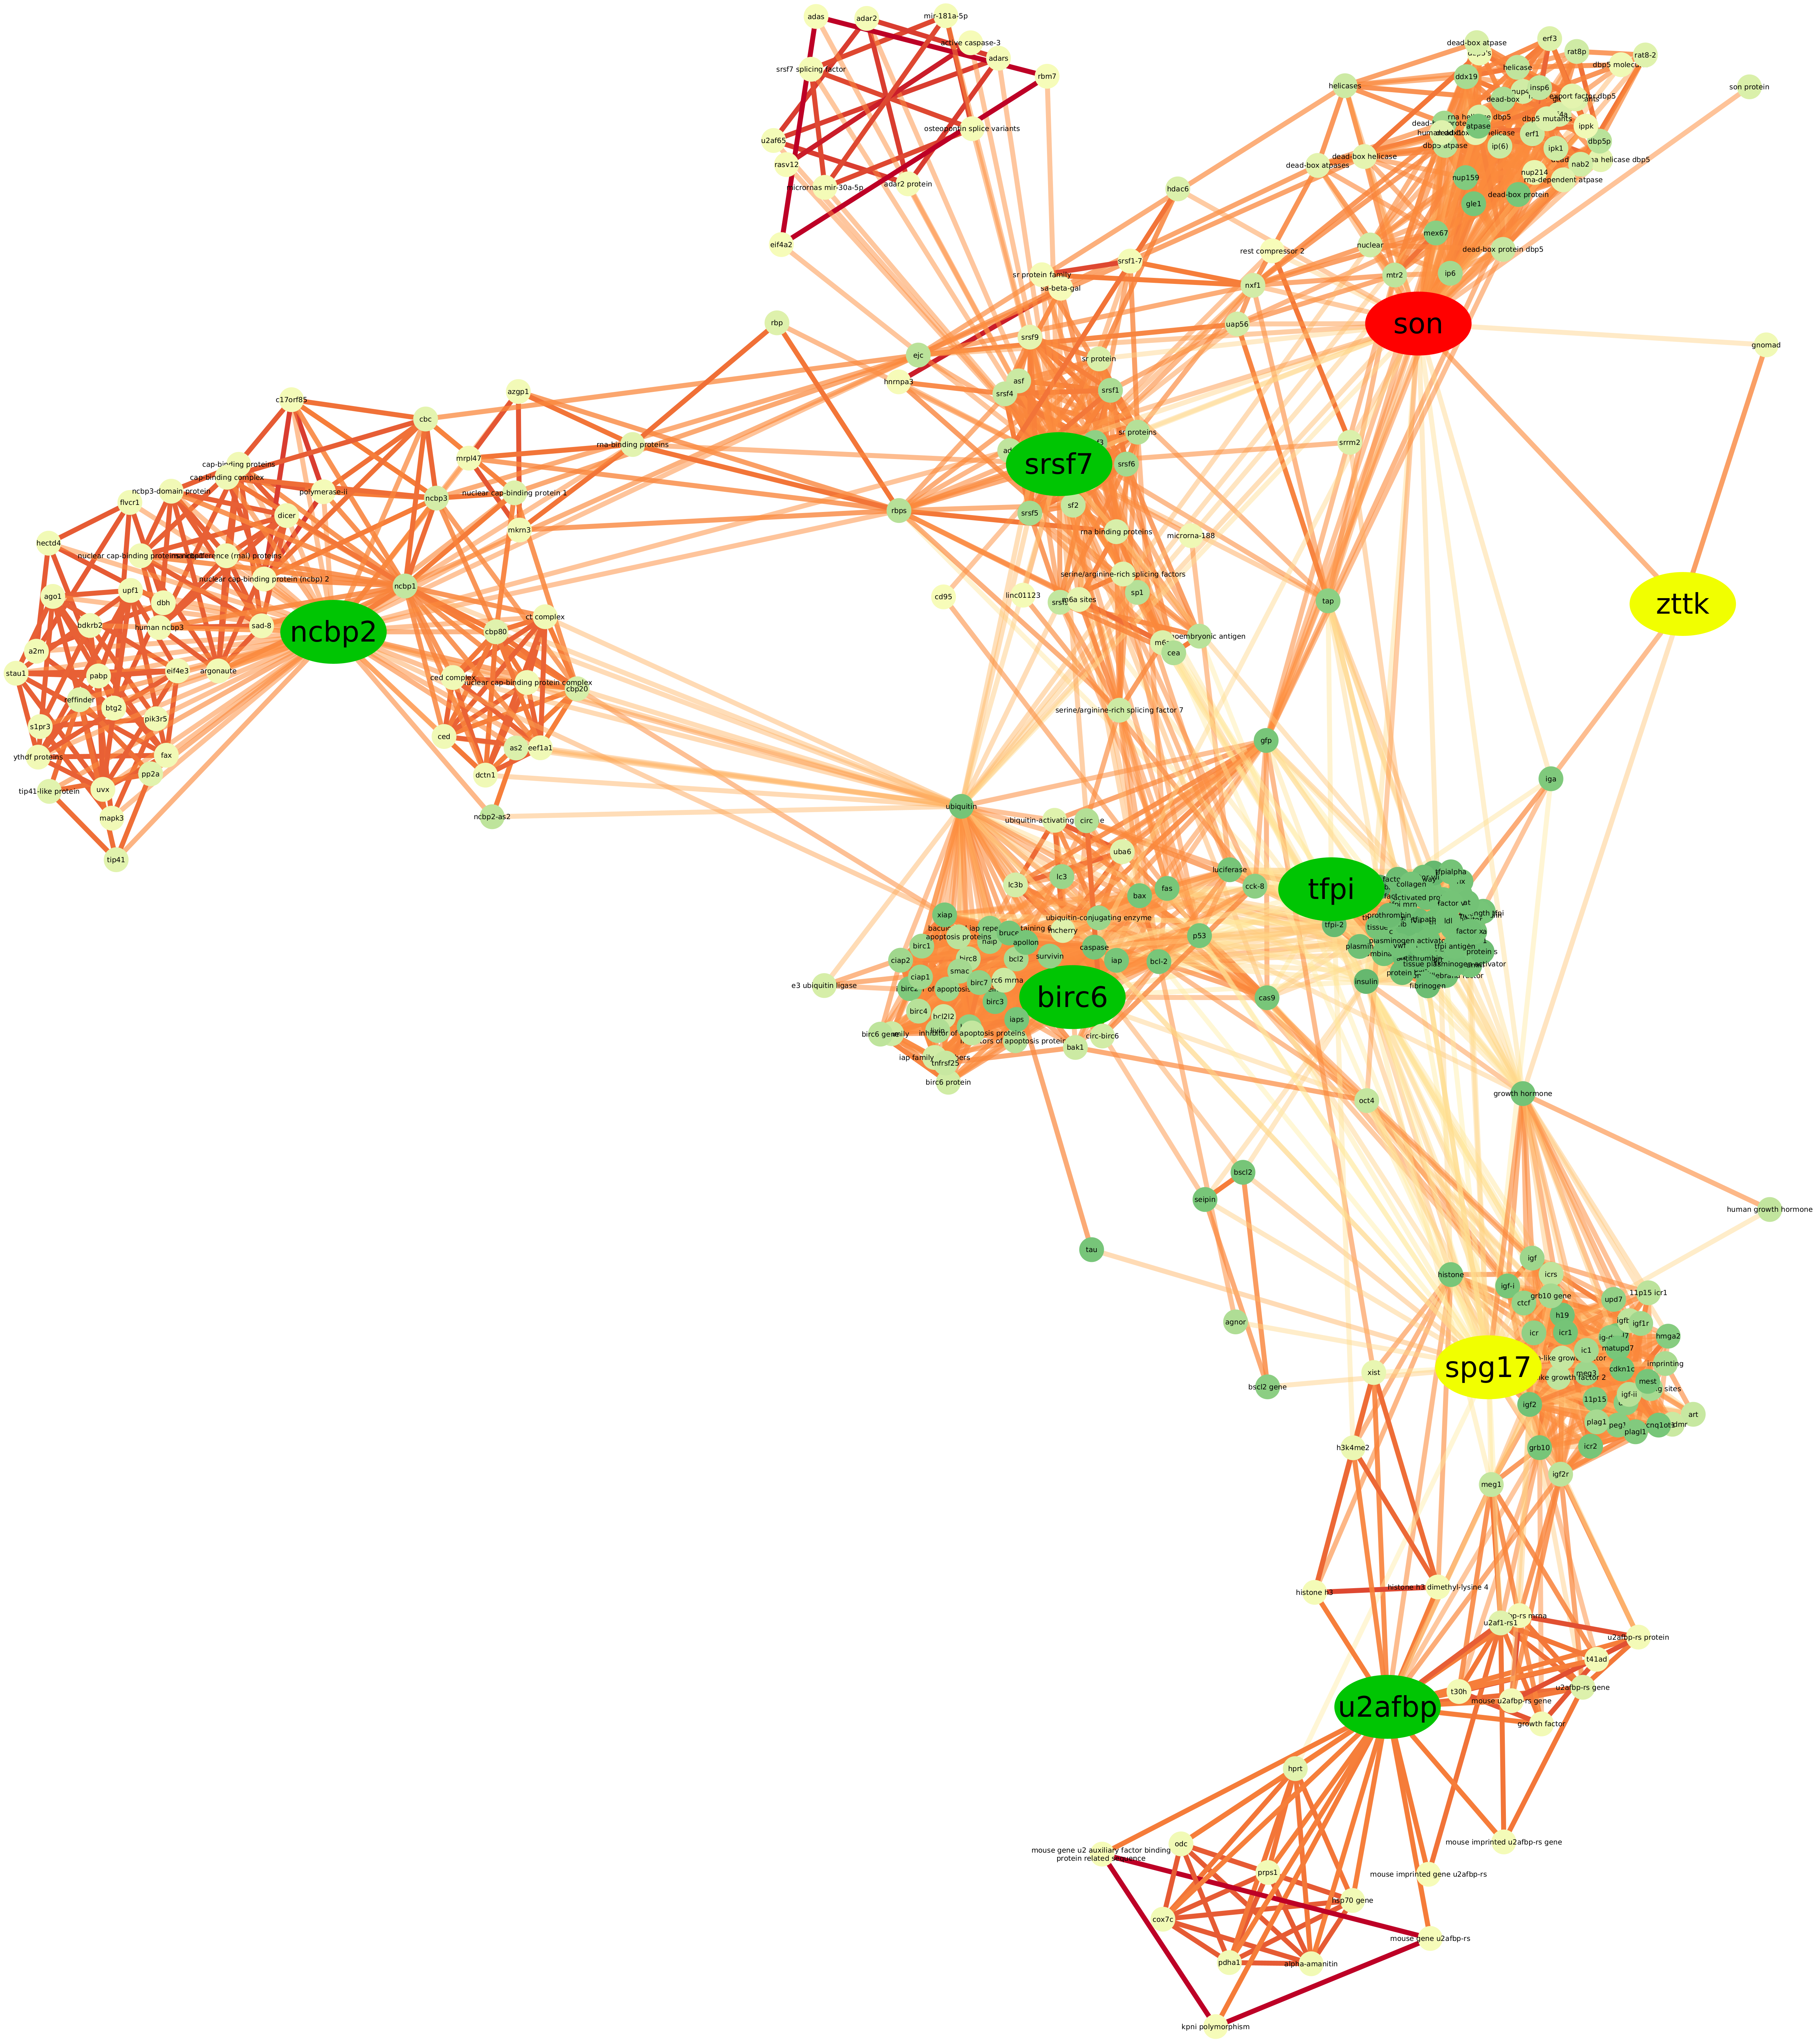
\includegraphics[width=\textwidth]{immagini/geni.png}
\caption{\footnotesize{Grafo ottenuto unendo i dataset sul gene SON (rosso), le due malattie causate dalla mutazione di SON: Zttk e Spg17 (giallo) e i cinque geni che interagiscono maggiormente con Son (verdi grandi). Gli altri nodi sono geni indotti dagli archi con capacità maggiore e sono colorati con una scala di verde proporzionalmente al loro numero di co-occorrenze. Gli archi sono colorati con una scala di rossi proporzionalmente al numero di co-occorrenze. Layout calcolato con l'algoritmo Fruchterman-Reingold delle forze dirette.}}
\label{fig:geni}
\end{figure}

Disegnando il grafo utilizzando gli stessi dati, ma normalizzato con CR2 abbiamo la figura \ref{fig:geni2}. In questo caso abbiamo forte tendenza dei cluster a rimanere isolati. Questo accade perché probabilmente i cluster contengono entità localmente rilevanti per il centroide ma non a livello globale, in aggiunta, le interazioni tra questi specifici geni sono evidentemente poco studiate in letteratura. Ciò nonostante rimane evidente almeno il legame tra Spg17 e u2afbp, portando quest'ultimo ad essere il più affidabile candidato \quotes{mediatore} tra SON e Spg17. Le osservazioni grafiche sono confermate dai dati nelle tabelle \ref{tab:geni_stat} e \ref{tab:geni2_stat}, che mostrano qualche statistica sui due grafi. Specificamente, il numero di nodi è quasi lo stesso mentre il numero di archi e il grado medio sono circa il quadruplo nel grafo \ref{fig:geni}.

\begin{figure}[!htb]
\centering
\includegraphics[width=\textwidth]{immagini/geni2.png}
\caption{\footnotesize{Grafo ottenuto unendo i dataset sul gene SON (rosso), le due malattie causate dalla mutazione di SON: Zttk e Spg17 (giallo) e i cinque geni che interagiscono maggiormente con Son (verdi). Gli altri nodi sono geni indotti dagli archi con capacità maggiore. Gli archi sono colorati con una scala di rossi proporzionalmente al numero di co-occorrenze. Layout calcolato con l'algoritmo Fruchterman-Reingold delle forze dirette.}}
\label{fig:geni2}
\end{figure}


\begin{table}[htb]
\parbox{.4\linewidth}{
\centering
\begin{tabular}{|l|l|}
    \hline
    \small{Nodi} & \small{331}	\\
    \small{Archi} &	\small{3105}\\
    \small{Grado medio} & \small{18.76} 	\\
    \small{Distanza media} & \small{2.9}	\\
    \small{Coefficiente di clustering} & \small{0.757}	\\
    \small{Densità} &	\small{0.067}\\
    \hline
\end{tabular}
\caption{\footnotesize{Statistiche riguardanti il grafo in figura \ref{fig:geni}.}}
\label{tab:geni_stat}
}
\hfill
\parbox{.4\linewidth}{
\centering
\begin{tabular}{|l|l|}
    \hline
    \small{Nodi} & \small{339}	\\
    \small{Archi} &	\small{781}\\
    \small{Grado medio} & \small{3.966} 	\\
    \small{Distanza media} & \small{3.54}	\\
    \small{Coefficiente di clustering} & \small{0.631}	\\
    \small{Densità} &	\small{0.017}\\
    \hline
\end{tabular}
\caption{\footnotesize{Statistiche riguardanti il grafo in figura \ref{fig:geni2}.}}
\label{tab:geni2_stat}
}
\end{table}

Nella figura \ref{fig:geni3} è stato usato il concetto di widest set (WS) definito nel paragrafo \ref{WS}, per identificare le entità che connettono maggiormente gli 8 concetti centrali: SON, Zttk, Spg17 e i 5 geni legati a SON. L'insieme dei nodi sorgente (NS) è composto proprio da questi 8 nodi, i dataset sono quelli relativi a queste entità. Il WS che ne risulta è composto dalle entità in tabella \ref{tab:WS_geni}, mentre tutti i singoli path calcolati sono riportati in tabella \ref{tab:WP_geni}. Per ogni nodo nel WS sono visualizzati i 30 geni indotti dagli archi con capacità maggiore usando CR2.

\begin{figure}[!htb]
\centering
\includegraphics[width=\textwidth]{immagini/geni3.png}
\caption{\footnotesize{I dataset usati sono SON, Spg17 e T5p, gli stessi delle figure \ref{fig:geni} e \ref{fig:geni2}. I nodi in magenta sono i geni che interagiscono con SON. I nodi verdi più grandi sono quelli nel aggiunti nel WS, per ognuno di essi sono stati aggiunti 30 geni indotti dagli archi con CR2 maggiore.}}
\label{fig:geni3}
\end{figure}

%Non abbiamo nessuna conoscenza per poter fare delle ipotesi in campo medico, 
Anche se estrarre delle ipotesi in campo medico necessiterebbe expertise specializzata, possiamo comunque analizzare la struttura del grafo e le entità incluse.  Osserviamo che spesso coppie o triplette di entità vanno a condividere parti di uno stesso cluster, per esempio Spg17 con histone e actin, che a sua volta ha un cluster in comune con tfpi, proteina che interagisce con SON ma che era rimasta un po' isolata nelle analisi precedenti, generando in questo modo dei ponti tra varie malattie.
I nodi totali, mostrati nella tabella~\ref{tab:geni3_stat}, sono relativamente pochi, perché il WP è passato spesso attraverso le stesse entità. Questo è confortante e indica che la metodologia è in grado di individuare delle entità rilevanti. Il grado medio, il coefficiente di clustering e la densità (stessa tabella~\ref{tab:geni3_stat}) sono significativamente più alti rispetto al grafo della figura \ref{fig:geni2}. Infatti dopo aver rimosso le entità condivise a favore di quelle più specifiche passando dal grafo nella figura \ref{fig:geni} al grafo nella figura \ref{fig:geni2}, le abbiamo reintrodotte attraverso il WS. Ripetendo l'operazione di selezione delle entità specifiche (con CR2) abbiamo trovato questa volta nodi che in realtà sono comuni.

\begin{table}[htb]
\parbox{.45\linewidth}{
\centering
\begin{tabular}{|l|l|}
    \hline
    \small{Nodi} & \small{410}	\\
    \small{Archi} &	\small{1300}\\
    \small{Grado medio} & \small{6.341} 	\\
    \small{Distanza media} & \small{3.420}	\\
    \small{Coefficiente di clustering} & \small{0.789}	\\
    \small{Densità} &	\small{0.016}\\
    \hline
    \end{tabular}
    \caption{\footnotesize{Statistiche riguardanti il grafo in figura \ref{fig:geni3}.}}
    \label{tab:geni3_stat}
}
\hfill
\parbox{.45\linewidth}{
\centering
    \begin{tabularx}{\linewidth}{|X|}
    \hline
    \scriptsize{'u2afbp', 'mkrn3', 'zttk', 'crp detection antibody', 'rest compressor 2', 'son', 'mll complex', 'microrna-500', 'c-reactive protein', 'ncbp2', 'human tissue factor pathway inhibitor gene', 'ezh2', 'rasv12', 'foetal brain proteins', 'spg17', 'birc6', 'antifactor (anti)-xa', 'speckle marker protein', 'luciferase', 'tfpi', 'sp1', 'srsf7', 'histone', 'actin', 'histone h3', 'long non-coding rna dleu1', 'sa-beta-gal'}\\
    \hline
    \end{tabularx}
    \caption{\footnotesize{Le entità del WS avente come nodi sorgenti: SON, Zttk, Spg17 e i geni che interagiscono con SON.}}
    \label{tab:WS_geni}
}
\end{table}

\begin{table}[!htb]
    \begin{tabularx}{\textwidth}{|l|l|X|}
            \hline
            \textbf{Origine} & \textbf{Destinazione} & \textbf{Percorso}  \\
            \hline
            \scriptsize{spg17} & \scriptsize{son} & \scriptsize{ ['spg17', 'foetal brain proteins', 'actin', 'speckle marker protein', 'son'] } \\ \hline
        \scriptsize{spg17} & \scriptsize{u2afbp} & \scriptsize{ ['spg17', 'foetal brain proteins', 'actin', 'speckle marker protein', 'son', 'full-length son', 'histone', 'histone h3', 'u2afbp'] } \\ \hline
        \scriptsize{spg17} & \scriptsize{srsf7} & \scriptsize{ ['spg17', 'foetal brain proteins', 'actin', 'speckle marker protein', 'son', 'rest compressor 2', 'srsf7'] } \\ \hline
        \scriptsize{spg17} & \scriptsize{tfpi} & \scriptsize{ ['spg17', 'crp detection antibody', 'c-reactive protein', 'antifactor (anti)-xa', 'tfpi'] } \\ \hline
        \scriptsize{spg17} & \scriptsize{ncbp2} & \scriptsize{ ['spg17', 'foetal brain proteins', 'actin', 'speckle marker protein', 'son', 'rest compressor 2', 'srsf7', 'active caspase-3', 'ezh2', 'mkrn3', 'ncbp2'] } \\ \hline
        \scriptsize{spg17} & \scriptsize{birc6} & \scriptsize{ ['spg17', 'crp detection antibody', 'c-reactive protein', 'antifactor (anti)-xa', 'tfpi', 'mir-500', 'luciferase', 'dleu1', 'birc6'] } \\ \hline
        \scriptsize{spg17} & \scriptsize{zttk} & \scriptsize{ ['spg17', 'foetal brain proteins', 'actin', 'speckle marker protein', 'son', 'zttk'] } \\ \hline
        \scriptsize{son} & \scriptsize{u2afbp} & \scriptsize{ ['son', 'full-length son', 'histone', 'histone h3', 'u2afbp'] } \\ \hline
        \scriptsize{son} & \scriptsize{srsf7} & \scriptsize{ ['son', 'rest compressor 2', 'srsf7'] } \\ \hline
        \scriptsize{son} & \scriptsize{tfpi} & \scriptsize{ ['son', 'rest compressor 2', 'srsf7', 'hnrnpa3', 'sp1', 'human tissue factor pathway inhibitor gene', 'tfpi'] } \\ \hline
        \scriptsize{son} & \scriptsize{ncbp2} & \scriptsize{ ['son', 'rest compressor 2', 'srsf7', 'active caspase-3', 'ezh2', 'mkrn3', 'ncbp2'] } \\ \hline
        \scriptsize{son} & \scriptsize{birc6} & \scriptsize{ ['son', 'rest compressor 2', 'srsf7', 'hnrnpa3', 'sp1', 'human tissue factor pathway inhibitor gene', 'tfpi', 'mir-500', 'luciferase', 'dleu1', 'birc6'] } \\ \hline
        \scriptsize{son} & \scriptsize{zttk} & \scriptsize{ ['son', 'zttk'] } \\ \hline
        \scriptsize{u2afbp} & \scriptsize{srsf7} & \scriptsize{ ['u2afbp', 'histone h3', 'histone', 'full-length son', 'son', 'rest compressor 2', 'srsf7'] } \\ \hline
        \scriptsize{u2afbp} & \scriptsize{tfpi} & \scriptsize{ ['u2afbp', 'histone h3', 'histone', 'full-length son', 'son', 'rest compressor 2', 'srsf7', 'hnrnpa3', 'sp1', 'human tissue factor pathway inhibitor gene', 'tfpi'] } \\ \hline
        \scriptsize{u2afbp} & \scriptsize{ncbp2} & \scriptsize{ ['u2afbp', 'histone h3', 'histone', 'full-length son', 'son', 'rest compressor 2', 'srsf7', 'active caspase-3', 'ezh2', 'mkrn3', 'ncbp2'] } \\ \hline
        \scriptsize{u2afbp} & \scriptsize{birc6} & \scriptsize{ ['u2afbp', 'histone h3', 'histone', 'full-length son', 'son', 'rest compressor 2', 'srsf7', 'hnrnpa3', 'sp1', 'human tissue factor pathway inhibitor gene', 'tfpi', 'mir-500', 'luciferase', 'dleu1', 'birc6'] } \\ \hline
        \scriptsize{u2afbp} & \scriptsize{zttk} & \scriptsize{ ['u2afbp', 'histone h3', 'histone', 'full-length son', 'son', 'zttk'] } \\ \hline
        \scriptsize{srsf7} & \scriptsize{tfpi} & \scriptsize{ ['srsf7', 'hnrnpa3', 'sp1', 'human tissue factor pathway inhibitor gene', 'tfpi'] } \\ \hline
        \scriptsize{srsf7} & \scriptsize{ncbp2} & \scriptsize{ ['srsf7', 'active caspase-3', 'ezh2', 'mkrn3', 'ncbp2'] } \\ \hline
        \scriptsize{srsf7} & \scriptsize{birc6} & \scriptsize{ ['srsf7', 'hnrnpa3', 'sp1', 'human tissue factor pathway inhibitor gene', 'tfpi', 'mir-500', 'luciferase', 'dleu1', 'birc6'] } \\ \hline
        \scriptsize{srsf7} & \scriptsize{zttk} & \scriptsize{ ['srsf7', 'rest compressor 2', 'son', 'zttk'] } \\ \hline
        \scriptsize{tfpi} & \scriptsize{ncbp2} & \scriptsize{ ['tfpi', 'human tissue factor pathway inhibitor gene', 'sp1', 'hnrnpa3', 'srsf7', 'active caspase-3', 'ezh2', 'mkrn3', 'ncbp2'] } \\ \hline
        \scriptsize{tfpi} & \scriptsize{birc6} & \scriptsize{ ['tfpi', 'mir-500', 'luciferase', 'dleu1', 'birc6'] } \\ \hline
        \scriptsize{tfpi} & \scriptsize{zttk} & \scriptsize{ ['tfpi', 'human tissue factor pathway inhibitor gene', 'sp1', 'hnrnpa3', 'srsf7', 'rest compressor 2', 'son', 'zttk'] } \\ \hline
        \scriptsize{ncbp2} & \scriptsize{birc6} & \scriptsize{ ['ncbp2', 'mkrn3', 'ezh2', 'active caspase-3', 'srsf7', 'hnrnpa3', 'sp1', 'human tissue factor pathway inhibitor gene', 'tfpi', 'mir-500', 'luciferase', 'dleu1', 'birc6'] } \\ \hline
        \scriptsize{ncbp2} & \scriptsize{zttk} & \scriptsize{ ['ncbp2', 'mkrn3', 'ezh2', 'active caspase-3', 'srsf7', 'rest compressor 2', 'son', 'zttk'] } \\ \hline
        \scriptsize{birc6} & \scriptsize{zttk} & \scriptsize{ ['birc6', 'dleu1', 'luciferase', 'mir-500', 'tfpi', 'human tissue factor pathway inhibitor gene', 'sp1', 'hnrnpa3', 'srsf7', 'rest compressor 2', 'son', 'zttk'] } \\
        \hline
    \end{tabularx}
\caption{\footnotesize{I path di massima portata calcolati, riferiti al grafo in figura \ref{fig:geni3}.}}
\label{tab:WP_geni}
\end{table}


\FloatBarrier
\section{Analisi olistica}
In questa sezione analizzeremo tutti i dataset disponibili (tabella \ref{tab:dataset}) che sono stati scelti dopo aver selezionato i migliori risultati provenienti da IPA, Malacard, Genecard e STRING (sezione \ref{conoscenze_partenza}).

Generando un grafo con tutti i dataset della tabella \ref{tab:dataset} otteniamo \numprint{93388} nodi e \numprint{1563732} archi; i nodi sono meno delle entità distinte perché i paper nei quali compare una sola entità non vengono considerati dato che con il metodo delle co-occorrenze non avrebbero senso.

Il grado medio del grafo è di circa 33 nonostante la maggior parte dei nodi abbia grado minore di 25 come si vede nella figura \ref{fig:isto_grado}, che mostra la distribuzione dei gradi dei nodi.

\begin{table}[!htb]
\begin{minipage}[b]{0.45\linewidth}
\centering
\includegraphics[width=\linewidth]{immagini/isto_grado.png}
\captionof{figure}{\footnotesize{Istogramma del grado dei nodi. Sulle ascisse il grado, sulle ordinate la percentuale di nodi.}}
\label{fig:isto_grado}
\end{minipage}
\begin{minipage}[b]{0.5\linewidth}
\centering
\begin{tabular}{|l|l|}
    \hline
    \textbf{Entità} & \textbf{Grado}\\
    \hline
    \small{hepatitis b virus} & \small{20486}\\
    \small{tumor} & \small{14645}  \\
    \small{hbv} & \small{13856} \\
    \small{mouse} & \small{9671} \\
    \small{hepatitis b} & \small{9322} \\
    \small{mice} & \small{8986} \\
    \small{hbsag} & \small{7733} \\
    \small{tfpi }& \small{7537} \\
    \small{tumors} & \small{7507} \\
    \small{cancer} & \small{7139} \\
    \small{oligodendroglioma} & \small{6652} \\
    \small{nucleotide} & \small{6621} \\
    \small{hbv infection} & \small{6511} \\
    \small{oligodendrogliomas} & \small{6393} \\
    \small{hbeag} & \small{6088} \\
    \small{amino acid} & \small{5720} \\
    \small{gliomas} & \small{5562} \\
    \small{hepatocellular carcinoma} & \small{5512} \\
    \small{rat} & \small{5312} \\
    \small{tissue factor} & \small{5163} \\
    \small{yeast} & \small{5145} \\
    \small{chronic hepatitis b} & \small{5084} \\
    \small{tissue factor pathway inhibitor} & \small{5069} \\
    \hline
    \end{tabular}
    \caption{\footnotesize{Le entità con grado maggiore.}}
    \label{tab:max_grado}
\end{minipage}\hfill
\end{table}
La media è aumentata da poche entità che hanno un grado molto maggiore alle altre. Queste entità (mostrate in tabella \ref{tab:max_grado}) sono quelle che appartengono ai dataset più grandi o che appaino spesso nei testi biomedici (es. mice, mouse, yeast, cancer) indipendentemente da quello che si sta studiando.

\subsection{Fenotipo}

Nella figura \ref{fig:tutto_fenotipo} mostriamo alcuni nodi di tipo disease della rete completa. Sono evidenziate le cinque malattie collegate a SON che stiamo studiando, più il gene SON stesso. Da ogni nodo principale (quelli più grandi nella figura) sono indotte 50 malattie attraverso gli archi di capacità CR2 maggiore. Si osserva come Spg17 e mental retardation hanno una forte relazione ciascuno con il suo insieme di sintomi specifico (rispettivamente a sinistra e destra) ma condividono anche moltissime manifestazioni fenotipiche tra loro e con Zttk e brain oligodendroglioma (i nodi centrali). Le entità condivise, come si nota dai colori, sono anche quelle che occorrono di più nel dataset e sono termini prettamente generali: nel cluster di Zttk/SON abbiamo dismorfismi, ritardi nello sviluppo e disabilità mentale mentre in quello di brain oligodendroglioma ci sono varie specializzazioni dell'entità di cancro. L'epatite b invece, non sembra avere forti tratti in comune con le altre entità principali. 

Nonostante i vertici siano molto collegati nella zona centrale, il grado medio del grafo resta molto basso a causa della normalizzazione CR2 degli archi che tende a risaltare entità specifiche per ogni centroide.

Anche se la Zttk è considerata una malattia rara, i suoi sintomi principali sono in realtà condivisi con molte altre malattie. Alcune di queste come per esempio sindrome di Down, autismo e sindrome di Beckwith-Wiedemann si sono presentate spesso nel corso delle analisi nonostante non siano presenti nelle query PubMed per ottenere i dataset. Il sospetto è che probabilmente almeno alcuni dei casi di Zttk siano stati scambiati con una di queste malattie fenotipicamente vicinissime, considerato anche che il primo articolo di PubMed collegato alla Zttk è del 2019.

\begin{figure}[!htb]
\centering
\includegraphics[width=\textwidth]{immagini/tutto_fenotipo.png}
\caption{\footnotesize{Grafo ottenuto utilizzando tutti i dataset. Per ognuno dei nodi evidenziati sono stati aggiunti al grafo i 50 nodi indotti dagli archi di capacità maggiore che rappresentano malattie. \'E stata usata CR2. Il colore dei nodi non evidenziati varia in una scala di verde proporzionalmente al numero delle co-occorrenze totali, quello degli archi in una scala di giallo-rosso proporzionalmente al numero di co-occorrenze tra le due entità.}}
\label{fig:tutto_fenotipo}
\end{figure}

\newpage
\subsection{Genotipo}

Utilizziamo gli stessi dati dell'analisi fenotipica ma come entità principali di partenza prendiamo, oltre alle 5 malattie, anche i 5 geni correlati a SON. Da ogni nodo principale sono stati indotti 20 geni correlati basandosi sulla CR2 degli archi. 

Il risultato è mostrato nella figura~\ref{fig:tutto_genotipo}.
Osserviamo che il grafo ottenuto ha un grado medio altissimo, riscontrabile anche osservando la zona centrale della figura dove si concentrano la grande parte dei nodi. Tre dei geni che interagiscono con SON (in giallo) sembrerebbero avere una forte relazione con Epatite b, brain oligodendroglioma e Spg17.

In quest'analisi vengono identificati anche i geni che collegano la malattia Zttk alle altre malattie (oltre a SON). Osserviamo la proteina Tau coinvolta nel corretto funzionamento dei neuroni, che sembra collegare Zttk a vari cluster di altre malattie. 

\begin{figure}[!htb]
\centering
\includegraphics[width=\textwidth]{immagini/tutto_genotipo.png}
\caption{\footnotesize{Grafo ottenuto utilizzando tutti i dataset. Per ognuno dei nodi più grandi sono stati aggiunti al grafo i 20 nodi indotti dagli archi di capacità maggiore che rappresentano geni. \'E stata usata CR2. Il colore dei nodi piccoli varia in una scala di verde proporzionalmente al numero delle co-occorrenze totali, quello degli archi in una scala di giallo-rosso proporzionalmente al numero di co-occorrenze tra le due entità.}}
\label{fig:tutto_genotipo}
\end{figure}

\begin{table}[htb]
\parbox{.45\linewidth}{
\centering
    \begin{tabular}{|l|l|}
    \hline
    \small{Nodi} & \small{252}	\\
    \small{Archi} &	\small{849}\\
    \small{Grado medio} & \small{6.738} 	\\
    \small{Distanza media} & \small{2.770}	\\
    \small{Coefficiente di clustering} & \small{0.606}	\\
    \small{Densità} &	\small{0.027}\\
    \hline
    \end{tabular}
    \caption{\footnotesize{Statistiche riguardanti il grafo in figura \ref{fig:tutto_fenotipo}}}
    \label{tab:tutto_fenotipo_stat}
}
\hfill
\parbox{.45\linewidth}{
\centering
    \begin{tabular}{|l|l|}
    \hline
    \small{Nodi} & \small{219}	\\
    \small{Archi} &	\small{1621}\\
    \small{Grado medio} & \small{14.8} 	\\
    \small{Distanza media} & \small{2.85}	\\
    \small{Coefficiente di clustering} & \small{0.725}	\\
    \small{Densità} &	\small{0.068}\\
    \hline
    \end{tabular}
    \caption{\footnotesize{Statistiche riguardanti il grafo in figura \ref{fig:tutto_genotipo}}}
    \label{tab:tutto_genotipo_stat}
}
\end{table}


\chapter{Conclusioni}

In questo lavoro, dopo aver fatto una revisione degli strumenti per affrontare le fasi tipiche del biomedical text mining, abbiamo scelto un approccio che combina alcuni di essi, sviluppando BioCograph, un tool di analisi automatica della letteratura. La particolare combinazione scelta, i.e. estrazione delle entità dagli articoli utilizzando BioBERT ed analisi delle co-occorrenze in forma di grafo, non ci risulta essere stata tentata in precedenza; anche se non utilizza strumenti come la relation extraction con BioBERT, o question answering, potrebbe lo stesso rivelarsi utile grazie ad un maggiore controllo sui dati grezzi.

Nella tesi abbiamo descritto BioCograph e sviluppato una pipeline di analisi, esemplificata su uno caso di studio relativo alla malattia Zttk. BioCograph ci ha permesso di studiare relazioni tra malattie diverse sia dal punto di vista fenotipico che genetico, partendo da una grande quantità di informazioni e selezionando le più importanti, tramite metodi della teoria dei grafi. I risultati sono incoraggianti, dato che le informazioni fenotipiche estratte in modo automatico corrispondono alle conoscenze sulle varie malattie.


L'utilizzo di BioCograph richiede una fase preliminare di espansione manuale delle conoscenze per definire le query da utilizzare per scaricare gli articolo PubMed. Questa fase è molto delicata, in quanto si potrebbero escludere involontariamente un insieme di documenti utili. Tramite la nostra analisi abbiamo anche notato una grande frammentazione della conoscenza nel campo biomedico. Per esempio nel paragrafo \ref{son_spg17} abbiamo visto che la correlazione tra SON e Spg17 è curata manualmente e riportata su Genecard ma ci sono pochissimi paper a riguardo, così come nel paragrafo \ref{genotipiche_son_spg17} abbiamo constatato che le interazioni tra geni prese dal database String non sono studiate in letteratura. In questo senso, un'eventuale versione successiva del software che vuole essere ancora più funzionale in maniere automatica, dovrà integrare e pesare le informazioni da molteplici fonti.

La fase di normalizzazione dei nomi si è dimostrata critica soprattutto per le entità poco studiate, che tendono ad essere chiamate con nomi non uniformi. Per questo, BioCograph potrebbe essere migliorato integrando i sistemi di normalizzazione allo stato dell'arte e lavorando poi con ID univoci.

Abbiamo notato che una normalizzazione degli archi più forte tende a evidenziare le relazioni specifiche e quindi si comporta meglio con algoritmi su grafi globali come il flusso massimo. D'altra parte lasciando le capacità degli archi come il numero effettivo di co-occorrenze un algoritmo come la massima portata è in grado di ripercorrere le relazioni più studiate in letteratura.  

I risultati avuti nel caso di studio con la sindrome Zttk ci sembrano significativi: quando c'è stata la possibilità di confrontare i dati ottenuti con quelli già noti (come nel caso fenotipico) BioCograph si è dimostrato affidabile e questo lascia sperare che possa essere così anche per eventuali nuove correlazioni genotipiche che sono emerse e che dovranno essere verificate da esperti della malattia.  

\printbibliography %Prints bibliography


\end{document}